\documentclass[10pt,a4paper]{report}
\usepackage[dvipsnames]{xcolor}
\usepackage{nag}
\usepackage{rotating}
\usepackage[autosize]{dot2texi}
\usepackage[Bjarne]{fncychap}
\usepackage{tikz}
\usetikzlibrary{shapes,arrows,decorations}
\usepackage{listings}
\usepackage{textcomp}
\usepackage{mathtools}
\usepackage{caption}

\DeclareCaptionFont{white}{ \color{white} }
\DeclareCaptionFormat{listing}{
  \colorbox[cmyk]{0.43, 0.35, 0.35,0.01 }{
    \parbox{\textwidth}{\hspace{15pt}#1#2#3}
  }
}
\captionsetup[lstlisting]{ format=listing, labelfont=white, textfont=white, singlelinecheck=false, margin=0pt, font={bf,footnotesize} }

% Language Definitions for SPARQL
\lstdefinelanguage{sparql}{
morestring=[b][\color{blue}]\",
morekeywords={SELECT,CONSTRUCT,DESCRIBE,ASK,WHERE,FROM,NAMED,PREFIX,BASE,OPTIONAL,FILTER,GRAPH,LIMIT,OFFSET,SERVICE,UNION,EXISTS,NOT,BINDINGS,MINUS,a},
sensitive=true
}

\colorlet{punct}{red!60!black}
\definecolor{background}{HTML}{EEEEEE}
\definecolor{delim}{RGB}{20,105,176}
\colorlet{numb}{magenta!60!black}

\lstdefinelanguage{json}{
    basicstyle=\normalfont\ttfamily\footnotesize,
    numbersep=8pt,
    showstringspaces=false,
    breaklines=true,
    literate=
     *{0}{{{\color{numb}0}}}{1}
      {1}{{{\color{numb}1}}}{1}
      {2}{{{\color{numb}2}}}{1}
      {3}{{{\color{numb}3}}}{1}
      {4}{{{\color{numb}4}}}{1}
      {5}{{{\color{numb}5}}}{1}
      {6}{{{\color{numb}6}}}{1}
      {7}{{{\color{numb}7}}}{1}
      {8}{{{\color{numb}8}}}{1}
      {9}{{{\color{numb}9}}}{1}
      {:}{{{\color{punct}{:}}}}{1}
      {,}{{{\color{punct}{,}}}}{1}
      {\{}{{{\color{delim}{\{}}}}{1}
      {\}}{{{\color{delim}{\}}}}}{1}
      {[}{{{\color{delim}{[}}}}{1}
      {]}{{{\color{delim}{]}}}}{1},
}

\lstset{frame=single,captionpos=b}


\title{Improving content discovery through combining linked data and data mining techniques}
\author{\vfill\textbf{Ross Fenning}}
\affil{
\vfill
  Dissertation submitted in partial fulfilment of the
\\
requirements for the degree of
\\
Master by Advanced Study in Software Engineering and Internet Architecture

\vfill


\textbf{School of Electrical Engineering \& Computer Science}
\\
\textbf{University of Bradford}
\vfill
}

\begin{document}

\maketitle

\begin{abstract}
\vfill
\noindent MSc in Software Engineering and Internet Architecture 2016
\vfill
\noindent Improving content discovery through combining linked data and data mining techniques
\vfill
\noindent By Ross Fenning
\vfill
\noindent Project Supervisor: Dr. D. Thakker
\vfill
\noindent A comparative study of multiple approaches for extracting linked data
from web content published by the BBC for the purposes of applying
machine learning to cluster related content.

This project designs and implements a process by which semantic data
about any piece of online media content can be extracted into RDF
models in
multiple ways and feature
sets for machine learning can be generated from
that data. The clusters produced by fourteen different permutations
of techniques are evaluated and a potential application of suggesting
related content is mocked up for qualititative evaluation.

It is concluded organisations can very easily make use of
embedded semantics within web pages due to better semantic properties
being made available in recent years because of pressure from
social media sites such as Facebook and Twitter.
These embedded semantics provide a good baseline for simple
learning that can group content based on broad categorisation.

However, feedback from the evaluation suggests that real value for
users from suggesting related content will come from linking items
based on topics and themes, which are better found via entity
extraction systems such as DBPedia Spotlight.

A simple application of entity extraction shows promising results in
evaluation and is highlighted as an area for organisations to explore
tuning to provide a powerful complement to embedded semantics.

\end{abstract}

\tableofcontents

\chapter{Introduction}
\label{chp:intro}

Media companies produce ever larger numbers of articles, videos,
podcasts, games, etc. -- commonly collectively known as ``content'' --
on the World Wide Web. A successful content-producing website not only
has to develop systems to aid producing and publishing that content,
but there are also demands to engineer effective mechanisms to aid
consumers in finding that content.

Approaches used in industry include providing a text-based search,
hierarchical categorisation (and thus navigation thereof) and even
more tailored recommended content based on past behaviour or content
enjoyed by friends (or sometimes simply other consumers who share your
preferences).

\section{Problems}
\label{sec:intro-problems}

There are several technical and conceptual problems with building
effective content discovery mechanisms, including:

\begin{itemize}

\item Large organisations can have content across multiple content
  management systems, in differing formats and data models.
  Organisations face large-scale enterprise integration problems
  simply trying to gain a holistic view of all their content.

\item Many content items are in fairly opaque formats, e.g. video
  content may be stored as audio-visual binary data with minimal
  metadata to display on a containing web page. Video content
  producers may not be motivated to provide data attributes that might
  ultimately be most useful in determining if a user will enjoy the
  video.

\item Content is being published continuously, which means any search
  or discovery system needs to keep up with content as it is published
  and process it into the appropriate data structures. Any machine
  learning previously performed on the data set may need to be re-run.

\end{itemize}

Many of these problems are felt within the BBC and are potentially
issues in many similar organisations. The BBC website officially
launched in 1997 and many articles from that year are still available
in archived form. Over the last 20 years, multiple content management
systems were created and retired such that today even the active
website is served by a mix of emerging, cutting-edge platforms and
systems that have been running for a number of years.

Technologies such as the World Wide Web and the maturity of the
media industry in its adoption in the last decade creates both an
opportunity to give consumers access to a substantial amount of
media content and a challenge in trying to make cohesive sense of
a diverse range of content, perhaps produced in an organistion that
was traditionally very fragmented as the BBC was.

\section{Hypothesis}

The following hypotheses are proposed for gaining new insights about
an organisation's diverse corpus of content:

\begin{itemize}

\item Research and software tools around the concept of
  \emph{Linked Data} can aid us in rapidly acquiring a broad view
  (perhaps initially at the expense of depth) of a organisation's
  content whilst also providing a platform for simple enrichment of
  that content's metadata.

\item We can establish at least a na\"ive mapping of an RDF graph
  representing a content item to an attribute set suitable for data
  mining. With such a mapping, we can explore applying machine
  learning -- particularly unsupervised learning -- across an
  organisation's whole content corpus.

\item Linked Data and Semantic Web \emph{ontologies} and models
  available can provide data enrichment beyond attributes and keywords
  explicitly avaiable within content data or metadata.

\item Many content-producers currently enrich their web pages with
  small amounts of semantic metadata to provide better presentation of
  that content as it is shared on social media. This enables simple
  collection of a full breadth of content with significantly less
  effort than direct integration with individual content management
  systems.

\end{itemize}

It is proposed also that all the data acquisition, enrichment and
mappings can be implemented in a general way when semantics and
linked data are used. The standardisations offered by the Semantic
Web and Linked Data research fields provides uniform interfaces and
patterns of data manipulation such that any software produced can be
applied to all of an organisation's content without consideration to
any particular class or type of item. This also does not preclude
including custom business rules later either, where domain experts
can give more guidance to treat data more intelligently.

The core principle in this research is that a generally-applicable
software system provides the best trade-off in terms of processing
the full breadth of content with the least amount of engineering
effort. This can allow media organisations to benefit from things
such as insights from machine learning across their whole corpus with
near-immediate results rather than embarking on large scale enterprise
integration projects over several months or years.

\chapter{Background}

This chapter discusses some of the existing research and technologies around
machine learning, RDF and combining them. It also covers some of the advantages
of using linked data and RDF in an enterprise setting and what tools and
approaches are well-defined enough that a corporation could build on top of
them rapidly.

Data mining activities such as machine learning rely on structuring data as
\emph{feature sets}\cite{bishop2006pattern} -- a set or vector of properties or
attributes that describe a single entity.
The process of \emph{feature extraction}
generates such feature sets from raw data and is a necessary early phase for
many machine learning activities.

The rest of this chapter will show:

\begin{enumerate}
\item that extracting feature sets from RDF\footnote{http://www.w3.org/TR/PR-rdf-syntax/} graphs can be done elegantly and follows naturally from some
previous work in this area; and
\item that the RDF graph is a suitable and even desirable data model for content
metadata in terms of acquiring, enriching and even transforming that data ahead
of feature extraction.
\end{enumerate}

\section{Data Mining}

TODO

\section{RDF and Feature Extraction}
\label{sec:rdf-and-features}

The RDF graph is a powerful model
for metadata based on representing knowledge as a set of
subject-predicate-object \emph{triples}. The query language, SPARQL, gives us a
way to query the RDF graph structure using a declarative pattern and return a
set of all variable bindings that satisfy that pattern.

For example, the SPARQL query in Listings~\ref{lst:sparqlfoaf}
queries an RDF graph that contains contact information and returns the
names and email address of all ``Person'' entities therein.

Notably, Kiefer, Bernstein and Locher\cite{kiefer2008adding} proposed a novel
approach called SPARQL-ML -- an extension to the
SPARQL\cite{segaran2009programming} query language with new keywords to
facilitate both generating and applying models. This means that the system
capable of parsing and running standard queries must also run machine learning
algorithms.

Their work involved developing an extension to the SPARQL query
engine for \emph{Apache Jena}\footnote{https://jena.apache.org/} that integrates
with systems such as \emph{Weka}\footnote{http://www.cs.waikato.ac.nz/ml/weka/}.
A more suitable software application for enterprise use might focus solely on
converting RDF graphs into a neutral data structure that can plug into arbitrary
data mining algorithms.

\begin{lstlisting}[label=lst:sparqlfoaf,caption={Example SPARQL query for people's names and email addresses},language=sparql]
PREFIX foaf: <http://xmlns.com/foaf/0.1/>
SELECT ?name ?email
WHERE {
  ?person a foaf:Person.
  ?person foaf:name ?name.
  ?person foaf:mbox ?email.
}
\end{lstlisting}

If we consider an RDF graph, $g$, to be expressed as a set of triples:

\begin{displaymath}
  (s, p, o) \in g
\end{displaymath}

\noindent this query could then be
expressed as function $f: G \rightarrow (S \times S)$ where $G$ is the set of
all possible RDF graphs and $S$ is a set of all possible strings.
This allows the result of the
SPARQL query to be expressed as a set of all SELECT variable bindings that
satisfy the WHERE clause:

$$
q(g,n,e) = \exists p . (p, type, Person) \in g\ \land (p, name, n) \in g \land (p, mbox, e) \in g
$$

$$
g \in G \models f(g) = \{(n, e) \subseteq (S \times S) \: | \: q(g,n,e)\}
$$

This could be generalised to express a given feature set as
vector $(a_1, a_2, ..., a_n)$:

$$
g \in G \models (a_1, a_2, ..., a_n) \in f(g)
$$

\noindent and in the case where all $a_k \in f(g)$ are literal (e.g. string or
numeric) values, we can thus consider a given SPARQL query to be specific
function capable of feature extraction from any RDF graph into sets of
categorical or numeric features.

\begin{lstlisting}[label=lst:sparqlabout,caption={SPARQL query to determine what },language=sparql]
PREFIX rdf: <http://www.w3.org/1999/02/22-rdf-syntax-ns#>
SELECT ?topic
WHERE {
  ?article rdf:about ?topic .
}
\end{lstlisting}

This might allow a query that extracts a country's population, GDP, etc.
provide feature extraction for learning patterns in economics, for example.
However, this is limited to features derived from single-valued predicates
with literal-valued ranges. It is not clear how to formulate a query that
expresses whether or not a content item is about a given topic.

In the RDF
model, it would be more appropriate to use a query like that in
Listings~\ref{lst:sparqlabout} where for a given $?article$ identified by
URI, we can get a list of URIs identifying concepts which the article mentions.
Such a query might be expressed as function $f': G \rightarrow \mathcal P(U)$ where $U$ is
set of all URIs such that:

$$
g \in G \models f'(g, uri) = \{t \: | \: (uri, about, t) \in g\}
$$

An approach of generating attributes for a given resource was proposed by
Paulheim and F\"urnkranz\cite{paulheim2012unsupervised}. They defined specific
SPARQL queries and provided case study evidence for the effectiveness of
each strategy.

Their work focused on starting with relational-style data (e.g. from a
relational database) and using \emph{Linked Open Data} to identify entities
within literal values in those relations and generated attributes from
SPARQL queries over those entities.

For a large content-producer, there is a more general problem where many content
items do not have a relational representation and the content source is a body
of text or even a raw HTML page. However, the feature generation from Paulheim
and F\:urnkranz proves to be a promising strategy given we can acquire an RDF
graph model for content items in the first place.

\section{RDF in the enterprise}
\label{sec:linked-enterprise-data}

\subsection{Data Fragmentation in Organisations}
\subsection{Enterprise Integration}
\subsection{Organisational Difficulties with Enterprise Integration}
\label{sec:ei-difficulties}
\subsection{Linked Enterprise Data}

\chapter{System Design}
\label{chp:design}

In this chapter, a system is inductively derived and concretely design to make
use of multiple strategies for:

\begin{enumerate}
\item gathering (meta)data about all of an organisations content items;
\item extracting metadata not explicitly modelled in source content management
systems;
\item further enriching that metadata with information not explicitly present
in the content item itself; and
\item applying machine learning to that content metadata to gain new insights
about that content.
\end{enumerate}

Initially, uses cases and a brief technical architecture for the
proposed system are given and then a theoretical data pipeline is
inductively defined that is the core proposition that extracts
semantics and prepares them for machine learning.

It is assumed that an organisation is already publishing its content
on HTML pages available on the public Internet and that engineers
can make use of existing machine learning algorithms and libraries. It
is out of the scope for the paper to deviate from well-established
machine learning techniques such as hierarchical clustering.

\section{Use Cases}
\label{sec:usecases}

Figure~\ref{fig:use-case} describes how a proposed ``Content Clustering''
software application would be used by established roles in a media
organisation.

\begin{sidewaysfigure}
  \begin{center}
    \includegraphics[width=\linewidth]{diagrams/usecase.png}
  \end{center}
  \caption{Use case diagram for content clustering system\label{fig:use-case}}
\end{sidewaysfigure}

The two main classes of user are those who \emph{produce} content,
e.g. journalists and TV programme makers, and those who will then
benefit from a potential application of these clusters -- in this case,
a feature is proposed that allows website users to find content related
to content they have just finished. These are the people that
\emph{consume} the output of the system.

Note that content production breaks down into several, differing
categories. In figure~\ref{fig:use-case}, we can see two examples of
a journalist writing news articles and a TV production team
publishing information about a particular episode or series. This is
by no means exhaustive as we may well have games developers creating
education games for children, editorial staff publishing recipes that
have appeared on cooking programmes aired by the BBC or pages
delivering the weather forecast for a particular city.

The audience members also break down into multiple categories who
could be reading news articles, watching programmes on on-demand
catch-up TV (e.g. BBC iPlayer) or a child reading educational materials.
These categories are depicted to remind there are multiple ways to
consume content as well as produce it, but it is also important to
note these roles can be transient if we are to promote content truly
on its relevance irrespective of the data store that happens to hold
it.

For example, a child or adult reading informative or educational
material may be interested in a relevant documentary available on
TV catch-up or somebody reading a news article about a topic might
wish to be informed that there are more in-depth educational guides
describing that topic in greater details (e.g. a press release about
a science discovery leading to a full, informative guide on that
field of science).

\section{High-Level Architecture}

The use cases depicted and described in Section~\ref{sec:usecases} naturally
lead to an application with two distinct interfaces: notification of new
content to consider for data mining and retrieval of information about content
clusters created to date.

\begin{figure}[h]
  \begin{center}
    \includegraphics[width=\linewidth]{diagrams/component.png}
  \end{center}
  \caption{High-level component diagram with interfaces for each use case\label{fig:component}}
\end{figure}

Figure~\ref{fig:component} shows a high-level view of a ``Content Miner''
software application that provides both interfaces. A set of ``notifier''
applications can be created to connect different content production and
management systems to the data mining system such that it is notified when new
content is created. The notification need only be an \emph{IRI} that uniquely
identifies that content item.

A \emph{Content Promotion Module} is also depicted as the example application
of the use case where website visitors or audience members then use the
data mining system to find content related to a page they are currently viewing.

The content miner breaks down into two general components: a pipeline
that prepares the data for machine learning and the clustering at the
end on that prepared data. The primary focus of this work is to
evaluate approaches for the former in the form of a
\emph{data pipeline} that uses semantics to take in a content item's
identifier at the source end and produces feature sets for data mining
at the output end. This data pipeline is inductively defined and
designed in the following section.

\section{Data Pipeline}
\label{sec:design-pipeline}

As stated in the previous section, a core subsystem in the overall
system is a conceptual data pipeline whose input is a URI or IRI
identifying a content item published on an organisation's website and
the output is feature sets ready for applying machine learning.

In this section, a theoretical pipeline is inductively defined in
steps such that an application of this pipeline would choose to
implement some subset of all potential pipeline stages as appropriate
for the relevant problem domain.

In Chapter~\ref{chp:implementation}, a system is engineered that implements
as many of these pipeline stages as possible such that a running instance of
the application can configure which components to use and which not to use.
Then in Chapter~\ref{chp:evaluation}, an evaluation of the system is given
while it is running each component in isolation to demonstrate which of the
theoretically-defined processes in this chapter appears to be most effective
in generating feature sets specifically for clustering web content.

\subsection{Definitions}

This system requires some initial definition of some data structures in use:

\begin{description}

\item[IRI] \hfill \\
The input to the system is a character string conformant to the
IRI syntax defined in RFC 3987\footnote{http://tools.ietf.org/html/rfc3987}.
This allows more generality offered by
URIs\footnote{http://tools.ietf.org/html/rfc3986} but is trivially made
compatible with systems that use URIs through the conversion algorithm defined
in section~3.2 of RFC 3987. Note that the public URL by which the public can
read or otherwise consume the content is a valid identifier, but we are not
restricted to that.

\item[Feature Set] \hfill \\
The final output of this data pipeline is a data structure
analogous to a relation or tuple per IRI fed into the system. Every IRI should
have a literal value against all possible columns or fields. For binary fields,
(e.g. the presence of absence of a concept tag), a more pragmatic structure
might be a list of tags positively associated with the IRI rather than
explicitly assigning $false$ to all tags to which the content item does not
pertain. This is analogous to a spare matrix when dealing with a large number
of dimensions.

\item[Named RDF Graph] \hfill \\
The structure used throughout most of the data pipeline
is that of an RDF graph. This is used for all the benefits outlined in
Section~\ref{sec:linked-enterprise-data} such as ease of transformation and
combining of data sets. Named graphs are used such that all data acquired
are keyed back to the IRI of the content item being processed. This also allows
all graphs to be combined in a \emph{triplestore} if needed to allow SPARQL
queries across the combined data for all content items. This can be modelled as
a data structure in many programming languages, but where a serialisation is
used (e.g. examples shown here or to send the data between components), the
JSON-LD\cite{sporny2014json} syntax will be used.
\end{description}

\subsection{Identity Graph}
\label{sec:identity-graph}

\begin{centering}
\begin{lstlisting}[label=lst:jsonld-identity,caption={Identity graph for a content item in JSON-LD syntax},language=json]
{
  "@id": "http://example.com/entity/1",
  "@graph": []
}
\end{lstlisting}
\end{centering}

With the knowledge only of a content item's IRI, we are arguably only able to
produce an empty named RDF graph. Such a graph for an example IRI
\texttt{http://example.com/entity/} is illustrated in
JSON-LD syntax in Listings~\ref{lst:jsonld-identity}.

The most na\"ive feature set we can generate from such an RDF graph is clearly
a singleton relation \texttt{("http://example.com/entity/")} where a single
$IRI$ field has the value \texttt{"http://example.com/entity/"}. It is also
clear that a set of one-dimension feature vectors with unique values in each
is not suitable for any form of machine learning activity. This does, however,
illustrate a baseline for a working software application that is -- at least
in the syntactic sense -- transforming IRI inputs to feature sets outputs.
Such a $null$ feature generator is depicted in Figure~\ref{fig:gen-null}.

\begin{figure}[h]
  \begin{center}
    \begin{dot2tex}[dot,options=-t math,autosize,pgf,scale=0.7]
      digraph g {
        rankdir=LR;

        node [shape=circle,margin="0,0"];
        edge [len=2];

        IRI -> RDF [label="extract"];
        RDF -> Features [label="(IRI)"];
      }
    \end{dot2tex}
  \end{center}
  \caption{Null feature generator \label{fig:gen-null}}
\end{figure}

Note that Figure~\ref{fig:gen-null} shows all three data structures involved
despite having no functional use. We can also see top-level definitions of the
process where we first \emph{extract} semantic information in RDF from a
content item identified by IRI and then \emph{generate} features therefrom.
More useful models can now be inductively defined by adding atomic
subcomponents that may each add value to the overall transformation.

There are three clear axes along which we can improve this pipeline:
\emph{extract} more RDF data knowing only an item's IRI,
expand or \emph{enrich} an existing RDF graph
and then improve how we \emph{generate} features for data mining.
In the first instance, we can consider the former and add
a single pipeline stage for expanding the RDF graph.

\subsection{RDF Extraction}
\label{sec:rdf-extraction}

Tim Berners-Lee outlined four rules\cite{berners2011linked} for Linked Data,
rule number three of which states ``When someone looks up a URI, provide useful
information, using the standards''. If we assume that many pages have embedded
some semantic web or RDF data, then a simple extraction strategy would be
to deference the content item's IRI via an HTTP GET and pass the content
to a parser capable of extracting RDFa, microformats, etc.

Many tools such as the RDFLib\footnote{https://github.com/RDFLib/rdflib}
provide functionality for taking a URL and returning an RDF graph of all data
found when fetching the resource it represents, so this is arguably an ideal
first choice in attempting to learn something about a content item from its
IRI.

\begin{figure}[h]
  \begin{center}
    \begin{dot2tex}[dot,options=-t math,autosize,pgf,scale=0.7]
      digraph g {
        rankdir=LR;

        node [shape=circle,margin="0,0"]

        IRI -> RDFa [label="dereference"];
        RDFa -> RDF [label="parse"];
        RDF -> Features [label="(IRI)"];
      }
    \end{dot2tex}
  \end{center}
  \caption{Semantic web data extraction\label{fig:gen-rdfa}}
\end{figure}

Figure~\ref{fig:gen-rdfa} depicts the pipeline with a simple dereference
step added. Note that the feature set generated is still the singleton
relation with only the IRI value. Thus the next step should be to add a step
that improves the feature set generation.

\subsection{Feature Set Generation}

Paulheim and F\"urnkranz\cite{paulheim2012unsupervised} described a number of
SPARQL queries for generating feature sets from RDF data, which could inspire
a simple query such as that shown in Listings~\ref{lst:simple-sparql}. This
query generates a boolean \texttt{true} value for any properties that match
and implies \texttt{false} for those that do not.

\begin{lstlisting}[label=lst:simple-sparql,caption={Generates field \texttt{content\_?p\_?v} with value \texttt{true}},language=sparql]
SELECT ?p ?v
WHERE { ?iri ?p ?v . }
\end{lstlisting}

As also noted by Paulheim
and F\"urnkranz, this overlooks the
\emph{open world assumption}\cite{russel2010artificial}. However, application
of clustering algorithms on binary data can employ asymmetric distance metrics
such as Jaccard similarity coefficient\cite{witten2005data}, which notably
avoids deriving similarity from negative values. That is, two content items
lacking a particular property will contribute no information about their
(dis)similarity. Thus we safely avoid inadvertently grouping together one item
that genuinely lacks the property with another that indeed has the property,
but we lack the positive assertion thereof in the data extracted.

\begin{figure}[h]
  \begin{center}
    \begin{dot2tex}[dot,options=-t math,autosize,pgf,scale=0.7]
      digraph g {
        rankdir=LR;

        node [shape=circle,margin="0,0"]

        IRI -> RDFa [label="derefernce"];
        RDFa -> RDF [label="parse"];
        RDF -> Features [label="content\_?p\_?v"];
      }
    \end{dot2tex}
  \end{center}
  \caption{Semantic web content extraction with basic SPARQL feature generation\label{fig:gen-rdfa-basic}}
\end{figure}

The basic pipeline in Figure~\ref{fig:gen-rdfa} can thus be augmented with this
basic feature extraction to produce the pipeline depicted in
Figure~\ref{fig:gen-rdfa-basic}.

\subsection{RDF Enrichment}

The third and final direction in which this data pipeline can be improved is
in terms of data enrichment. A simple strategy here is to repeat the
dereferencing used in Section~\ref{sec:rdf-extraction}, but for each IRI
found as the object of a triple in which the initial IRI is the subject.
Formally:

$$
g \in G \models \exists p, o . (IRI, p, o) \in g \rightarrow g' = deref(o)
$$

That RDF graphs can be modelled as mathematical sets as in
Section~\ref{sec:rdf-and-features} means we can express a graph enriched this
way as a \emph{union} of the initial graph with each graph returned from all
dereferencing:

$$
g \in G \models g' = g \cup \bigcup \: \{deref(o) \: | \: (IRI, p, o) \in g\}
$$

Figure~\ref{fig:object-deref} shows the data pipeline with this additional
enrichment stage. Note that now we have potential for some stages being
executed in parallel.

\begin{sidewaysfigure}[h]
  \begin{center}
    \begin{dot2tex}[dot,options=-t math,autosize,pgf,scale=0.7]
      digraph g {
        rankdir=LR;

        node [shape=circle,margin="0,0"];

        dummy [shape=none,label=""];

        IRI [label="IRI"];
        RDF1 [label="RDF_1"];
        RDF2 [label="RDF_2"];
        RDFp [label="RDF'"];

        IRI -> RDFa [label="dereference"];
        RDFa -> RDF [label="parse"];
        RDF -> RDF1 [label="dereference/parse"];
        RDF -> RDF2 [label="dereference/parse"];
        RDF -> RDFp [label="\cup"];
        RDF1 -> RDFp [label="\cup"];
        RDF2 -> RDFp [label="\cup"];
        RDFp -> Features [label="content\_?p\_?v"];
      }
    \end{dot2tex}
  \end{center}
  \caption{\label{fig:object-deref}Semantic web content miner with additional dereferencing of linked entities}
\end{sidewaysfigure}

So far in this section, we have inductively built up a data pipeline from
a ``null'' base working with only identity graphs to a simple pipeline
capable of \emph{extracting} an RDF graph, \emph{enriching} it and then
\emph{generating} features from it.

What needs to be proven through experimentation is \emph{which} of these
provides the information required for effective data mining. As part of this
experimentation, we can now look at further techniques and approaches to try.

\subsection{Improving Extraction}

In order to gain a larger set of RDF data at the start of the pipeline, we
can derive further ways to get information about a content item given only
its IRI as input.

Rizzo and Troncy\cite{rizzo2012nerd} defined a framework called NERD capable
of combining multiple entity extraction systems to provide a unified way of
identifying -- and disambiguating -- named entities within a given body of text.
With such a system, we can create a second, parallel RDF extraction strategy
that creates a graph of triples in the form:

$$
(IRI, rdf\!\!:\!\!about, Entity)
$$

\noindent where $Entity$ is an IRI representing a concept or entity believed
to be found in the content's textual content. A data pipeline complementing
the RDFa-based extraction is depicted in Figure~\ref{fig:entity-extraction}.
Note the ability to apply a simple set union to the result of each extraction
as with the enrichment.

\begin{sidewaysfigure}[h]
  \begin{center}
    \begin{dot2tex}[dot,options=-t math,autosize,pgf,scale=0.8]
      digraph g {
        rankdir=LR;

        node [shape=circle,margin="0,0"]
        RDF1 [label="RDF_1"];
        RDF2 [label="RDF_2"];

        IRI -> RDFa [label="dereference"];
        IRI -> Text [label="GET"];
        RDFa -> RDF1 [label="parse"];
        Text -> RDF2 [label="entity extraction"];
        RDF1 -> RDF [label="\cup"];
        RDF2 -> RDF [label="\cup"];
        RDF -> Features [label="content\_?p\_?v"];
      }
    \end{dot2tex}
  \end{center}
  \caption{Named entity extraction in addition to semantic web extraction\label{fig:entity-extraction}}
\end{sidewaysfigure}

Another strategy can be to infer a relationship between two content items where
one contents an HTML link to another. It is not always possible to derive
precise semantics of such a link (unless the publisher has kindly provided
a \texttt{rel} attribute), but a weak relationship such as:

$$
(IRI_1, ex:related, IRI_2)
$$

\noindent might prove -- through experimentation -- to be useful enough
for data mining insights.

The fourth and final extraction strategy explored is acquiring metadata from
bespoke Content Management Systems and other internal APIs. This is generally
the only option used in enterprises settings, as discussed in
Section~\ref{sec:linked-enterprise-data}. This is likely to be the richest
source of information where an enterprise has typically preferred bespoke
integrations against non-hypermedia interfaces, so experimentation should
help quantity or qualify the value such a direct integration adds (perhaps to
consider it in combination with the cost of bespoke, repeated integration
projects).

The assertion explored here is that such bespoke integrations can
\emph{complement} cheaper work such as extracting RDFa with pre-built tools
(and thus be developed one-by-one after the initial release of an application
such as this data pipeline). Note that repeated custom integration projects
means that each data source requires a different application be developed (as
opposed to the reuse of a single RDFa parser or HTML link scraper). This
also means we are not necessarily comparing like-for-like if we introduce only
one at a time. It also makes it
difficult to evaluate data mining of a diverse content corpus if an integration
against an API provides additional metadata for only, say, 10\% of that corpus.

These challenges aside, it is clear that bespoke integrations have a clear place
in this data pipeline being applied in a real enterprise setting. Now that
we have a complete set of theoretical stages for \emph{extraction}, the
remaining improves lie now in the \emph{enrichment} and
\emph{feature generation} stages.

\subsection{Improving Enrichment}

In addition to enriching through dereferencing linked entities, it is proposed
to explore the following options:

\begin{itemize}
\item inferring relationships to hypernyms as defined by Wordnet\cite{miller1995wordnet};
\item inferring facts based using rules derived from expert domain knowledge;
\item using RDFS and OWL to generate new triples with well-established Ontology rules.
\end{itemize}

In the first approach, we can consider a relationship rule such as:

$$
(IRI, ex:related, ex:Dog)
$$

\noindent and \emph{infer} the fact:

$$
(IRI, ex:related, ex:Animal)
$$

\noindent and produce an enriched graph containing all additional facts
inferred in this way.

When dealing with proper nouns and named entities, inferring facts based on
domain knowledge may be more appropriate. For instance, the rule in n3 syntax:

\begin{lstlisting}
  {
    ?article ex:takesPlaceIn ?city .
    ?city a ex:City .
    ?city ex:capitalOf ?country .
  } -> { ?iri ex:takesPlaceIn ?country }
\end{lstlisting}

\noindent might be useful to help cluster articles that take place in the same
country -- even if the countries are not always explicitly mentioned therein.
Such an inference requires knowledge about cities and countries to
write and domain experts for different types of content might be able to offer
more nuanced rules.

An example for BBC content might be to infer that all articles written under
the \emph{Newsround} brand is suitable for children or that programmes that
have broadcast times during the day are also suitable for children.

The third and final proposed improvement makes use of standard tools to find
\emph{closures} using, e.g. RDFS, ontology rules. With this approach, we
can infer that entities that have a given type or class also have their
superclasses and supertypes. This gives us similar inference to hypernyms,
but with knowledge present in well-established ontologies.

An obvious example might where two content items have been identified as
related to the same concept -- so they would be candidates for clustering
together -- but when RDF data are extracted, it is found that two
different URIs have been used for each:

\begin{displaymath}
(IRI_{1}, <\!\!http\!:\!\!//dbpedia.org/property/related\!\!>, ex1:entity)\\
\end{displaymath}
\begin{displaymath}
(IRI_{2}, <\!\!http\!:\!\!//dbpedia.org/property/related\!\!>, ex2:anotherEntity)
\end{displaymath}

In the RDF graph for $IRI_2$, say, we might find the source had provided an
\texttt{owl:sameAs} assertion such as:

\begin{displaymath}
(ex2:anotherEntity, owl:sameAs, ex1:entity)
\end{displaymath}

This is possible in the case where the second item's data source uses its own
set of identifiers for entities, but has chosen to provide equivalences to
a more standard set of identifiers (e.g. DBpedia). With this information,
our data pipeline can infer:

\begin{displaymath}
(IRI_{1}, <\!\!http\!:\!\!//dbpedia.org/property/related\!\!>, ex1:entity)\\
\end{displaymath}
\begin{displaymath}
(IRI_{2}, <\!\!http\!:\!\!//dbpedia.org/property/related\!\!>, ex2:anotherEntity)\\
\end{displaymath}
\begin{displaymath}
(IRI_{2}, <\!\!http\!:\!\!//dbpedia.org/property/related\!\!>, ex1:entity)
\end{displaymath}

\noindent and the feature generation stage might provide the common features
\texttt{dbprop\_related\_ex1\_entity=true} for both content items.

\subsection{Improving Feature Generation}

The feature generation outlined so far relies solely on boolean values
indicating whether or not a given content item is related by some property to
some entity. This recreates the concept of \emph{tagging} where a given
object is either associated or not associated with a series of \emph{tags}.

One of the advantages of the RDF graph model is that we are not constrained
necessarily to properties and attributes directly applicable to the entity. We
could imagine adding a level of indirection to the query in
Listings~\ref{lst:simple-sparql} to create the query in
Listings~\ref{lst:level2-sparql}.


\begin{lstlisting}[label=lst:level2-sparql,caption={Generates field \texttt{content\_?p1\_?p2\_?v} with value \texttt{true}},language=sparql]
SELECT ?p1 ?p2 ?v
WHERE {
  ?iri ?p1 ?o .
  ?o ?p2 ?v .
}
\end{lstlisting}

With the this query, features of the form \texttt{content\_?p1\_?p2\_?v} can
be generated. An example of this might be where a television programme
content item has information about the actors that appeared therein, e.g.
\texttt{ex:hasActor}, and furthermore we have information about those actors
such as where they were born, e.g. \texttt{ex:bornIn}. With the path created
by following both of these predicates, it is possible to create features for
a television programme such as
\texttt{content\_ex:hasActor\_ex:bornIn\_Edinburgh} and we can potentially
find similarity between programmes where the actors were born in the same
city.

Perhaps a third step in the predicate path followed can give us even more
useful features. The example above could be expanded to
\texttt{content\_ex:hasActor\_ex:bornIn\_ex:cityIn\_Scotland} to allow the
more general ability to cluster programmes with Scottish actors, for instance.

Appropriate experimentation should show whether more value is gained by
adding these additional levels of indirection.

\subsection{Maximal Data Pipeline}

In this section, a data pipeline was inductively built up from a base,
identify pipeline with suggestions for potential improvements in different
stages. An application of all the ideas discussed so far might look like
that depicted in Figure~\ref{fig:maximal-pipeline}.

\begin{sidewaysfigure}[p]
  \begin{center}
    \begin{dot2tex}[dot,options=-t math,autosize,pgf,scale=0.8]
      digraph g {
        rankdir=LR;

        node [shape=circle,margin="0,0"]
        RDF1 [label="RDF_1"];
        RDF2 [label="RDF_2"];
        RDF3 [label="RDF_3"];
        RDFp [label="RDF'"];
        RDFp1 [label="RDF'_1"];
        RDFp2 [label="RDF'_2"];
        RDFp3 [label="RDF'_3"];
        RDFp4 [label="RDF'_4"];

        IRI -> RDF1 [label="\text{parse}"];
        IRI -> RDF2 [label="\text{extract}"];
        IRI -> RDF3 [label="\text{scrape}"];

        RDF1 -> RDF [label="\cup"];
        RDF2 -> RDF [label="\cup"];
        RDF3 -> RDF [label="\cup"];

        RDF -> RDFp1 [label="\text{dereference/parse}"];
        RDF -> RDFp2 [label="\text{hypernym inference}"];
        RDF -> RDFp3 [label="\text{expert inference}"];
        RDF -> RDFp4 [label="\text{OWL inference}"];

        RDF -> RDFp [label="\cup"];
        RDFp1 -> RDFp [label="\cup"];
        RDFp2 -> RDFp [label="\cup"];
        RDFp3 -> RDFp [label="\cup"];
        RDFp4 -> RDFp [label="\cup"];

        RDFp -> Features [label="\text{content\_?p\_?v}"];
        RDFp -> Features [label="\text{content\_?p1\_?p2\_?v}"];
      }
    \end{dot2tex}
  \end{center}
  \caption{\label{fig:maximal-pipeline}Maximal Data Pipeline}
\end{sidewaysfigure}

The goal of this work is to evaluate how the quality of unsupervised clustering
changes with respect to enabling different combinations of the maximal
data pipeline. In the next section, some of the technical architecture of this
pipeline is outlined and the next chapter will cover how the overall system is
then implemented.


\chapter{Implementation}
\label{chp:implementation}

In this chapter, some of the details of the system implementation
are described. Initially, we discuss some of the implementation
strategy employed due the experimental nature of the system and the
desire to run multiple, competing approaches side-by-side in an
efficient way.

The remaining sections walk through the implementation of each part
of the data pipeline from upstream to feature sets and the chapter
concludes with implementation of the clustering and generation of
clusters for evaluation.

\section{Software Architecture}

All functionality was implemented as part of a single Python module
named \emph{distillery}
that is run via the Unix command line, with different subcommands for
each feature. Each command was designed around the
Unix Philosophy\cite{raymond2003art} of doing one job per command and
that they were composable via Unix pipes. This allows pipelines to
be composed:

\begin{centering}
  \begin{lstlisting}[
      basicstyle=\scriptsize,
      label=lst:unix-pipe,
      language=bash]
distillery extract <iris.txt | distillery enrich | distillery generate
  \end{lstlisting}
\end{centering}

\noindent that resemble the entire theoretical data pipeline described
in section~\ref{sec:design-pipeline} without the need for middleware
such as message queues. More typical enterprise architectures around
message oriented middleware or event-driven architecture might need
to be employed to scale this system to millions of documents, but
the simple approach above is sufficient for tens of thousands of
documents.

Even this simple approach would scale very well with suitably low
network latency. The largest bottleneck observed was the necessity
to do at least one HTTP request per item ingested and then enrich
via an HTTP request per object of a triple where the IRI is a subject.
For some content items, this could easily be over 100 HTTP requests at
which point parallel CPU cores or asynchronous I/O programming does
not overcome the demands on network performance.

Throughput is a particular challenge when data processing systems
are first launched. The day-to-day volume of item creations and
updates may be low enough for even a low-scale application, but the
performance demands increase significantly when we wish to bootstrap
a backlog of all content items historically published -- of which
could easily be tens of millions for organisations such as the BBC.

For this, there is an
appeal to designing such a system on a cloud computing platform such
that it can be scaled up for the initial import of existing data and
then back down for ongoing updates when that import completes. Such
design is out of scope for this paper, but some discussion of
limitations of the existing system in section~\ref{} highlights where
this system may be architected differently to be more suitable for
such a cloud-based deployment.

The higher-level compositional architecture of the individual
data processing stages can, of course, be altered independently of
the design of those stages. The following sections will describe in
greater detail those composable modules.

\section{Avoiding Redundancy Across Multiple Experiments}

The design of the data pipeline in chapter~\ref{chp:design} would
suggest an implementation with each stage implemented as a function
converting a graph into a new, richer graph.

That is, whilst the different strategies illustrated in the maximal
data pipline in Figure~\ref{fig:maximal-pipeline} can be run in
parallel, the extraction stage itself simply converts the identity
graph described in section~\ref{sec:identity-graph} to a single graph
(after having taken the union of all the strategies).

In the experiment that is the subject of this paper, the intent was
to compare each of the extraction strategies individually, but also
all possible (union) combinations thereof. This presents at least
two potential implementation strategies:

\begin{enumerate}
\item Build the whole data pipeline and machine learning system such
  that it is configurable which strategies are invoked and run an
  instance per configurable combination; or
\item implement the software to produce all possible outcomes along
  the pipeline.
\end{enumerate}

The former approach is stronger if the aim is to build the system
closer to how it would be implemented in an enterprise: only one
set of clusters is needed and even a production, enterprise system
would be configurable if maintainers wished to enable or disable
features as desired.

The latter strategy is arguably better for experimentation as every
IRI fed into the source end of the pipeline is processed at the same
time for every extraction and enrichment approach. This gives better
assurance that the same input is used to evaluate each competing
system.

Other operational reasons include being able to run the system on a
single machine if necessary and that there is no repeated work:
extraction by one means can be used in isolation, but also feed into
a union with another technique without having to recalculate that
graph. That is, if we have graphs $A$ and $B$ generated once each,
then we can output $A$, $B$ and $A \cup B$ for comparison. A parallel copy
of each system would be calculating $A$ and $B$ twice each.

The limitation here is a production-ready implementation of the
system would have be built again from the ground-up, perhaps reusing
functions and library code from the experimental version, as the
application itself will be structured around this idea of multiple
outputs for each input. This is likely to be the case for any
experimental system and is arguably in line with Brooks' classic
assertion to ``Plan to Throw One Away''\cite{brooks1995mythical}.

\begin{centering}
  \begin{lstlisting}[
      label=lst:extract-all,
      language=python,
      caption={Python function that generates all possible RDF Graphs}]
def all_extracted_graphs(iri):
    
    extraction_strategies = [
        dereference, extract_entities, find_links
    ]

    # This creates all 3 RDF Graphs only once
    graphs = [s(iri) for s in extraction_strategies]

    # Empty set removed from powerset
    for idx, gs in enumerate(powerset(graphs) - {{},}):
        # union defined elsewhere: list(graph) -> graph
        graph = reduce(union, gs)
        # Loop counter idx tells us from which technique
        # combination each graph comes
        yield idx, graph
  \end{lstlisting}
\end{centering}

An illustrative Python function is shown in
Listings~\ref{lst:extract-all} where each of the three extraction
techniques is invoked only once and a powerset function is used to
generate all possible unions of those graphs and thus yield all
possible usages or non-usages of each strategy to generate RDF
graphs. The details of the three extraction functions are covered in
section~\ref{impl-extraction}.

\section{Obtaining IRIs}

It is a substantial undertaking to design, build and test a
production-quality enterprise system that processing all content
produced by a media organisation. An experimental system needs to
focus on quick results and therefore is optimised to work only over
a small sample of that content.

As introduced in section~\ref{intro-problems}, all that content is
also likely to be distributed across multiple databases, content
management systems and other stores. Whilst it is hypothesised in
this research that semantics and linked data provide a good way to
extract data about the total breadth of all content without any
bespoke integration against internal systems, there still remains
the enterprise integration problem of \emph{discovery} of those
content items.

Essentially, the data pipeline outlined in
section~\ref{sec:design-pipeline} notably requires that known IRIs of
content items are fed into it, but makes no statement about how those
IRIs are acquired. This is a deliberate design decision to decouple
the concepts of discovery from this extraction/enrichment workflow.
Thus item may easily be re-ingested several times if it is updated
(or simply periodically) and
a modular approach like this defends against upstream systems changing
and having to rebuild the triggers that notify when content is created
or updated.

What follows it that the enterprise integration task has been reduced
(we do not need to write bespoke code to extract basic data about
every content item) but not wholly eliminated (some custom adaptors
need to be created to notify the pipeline of creation or update events
in each respective data store).

However creation of any such notification adaptors is out of scope
for this research altogether, so a heuristic approach was employed
where ten different, themed content aggregation pages on the BBC
website\footnote{
  Including, among others, the BBC Homepage (http://www.bbc.co.uk),
  BBC Arts (http://www.bbc.co.uk/arts) and BBC Science
  (http://www.bbc.co.uk/science)
} were polled for any new content promoted by editorial teams.
This provided a way to find new items shortly after they are published
and also ensured the data sample ultimately used focused on content
that was deemed noteworthy or interesting in the last few months.

This is not an effective method for obtaining a large number of items
quickly as it is entirely dependent on the rate these aggregate pages
are updated. Running slowly over a long period yielded approximately
ten thousand individual IRIs with little effort nor need for large
amounts of integration work.

\section{Extracting RDF Graphs}
\label{sec:impl-extraction}

Listings~\ref{lst:extract-all} hinted at three individual functions
capable of obtaining an RDF graph for a given IRI, all based on the
extraction strategies outlined in section~\ref{sec:rdf-extraction}.

\subsection{Dereferencing}

Listings~\ref{lst:deref-simple} shows how trivial a dereference
function can be if we use the comprehensive RDFLib library for
Python. The library can handle content type
negotiation\cite{fielding2014hypertext} to ensure it can happily
dereference and parse any response that contains semantics,
particularly RDFa (including embedded Turtle) and microdata within an
HTML page.

\begin{centering}
  \begin{lstlisting}[
      label=lst:deref-simple,
      language=python,
      caption={Python function that generates all possible RDF Graphs}]
from rdflib import Graph
    
def dereference(iri):
    g = Graph(identifier=iri)
    g.parse(iri)
    return g
  \end{lstlisting}
\end{centering}

\subsection{Entity Extraction}
\label{sec:impl-entity-extraction}

DBPedia Spotlight\cite{isem2013daiber} was chosen to perform the
entity extraction. A hosted version is available as a free service and
it has been shown to be effective in many cases. A true comparative
study of the merits of alternative entity extractors is out of scope
for this paper.

\begin{centering}
  \begin{lstlisting}[
      label=lst:extract-entities,
      language=python,
      caption={Python function that uses DBPedia Spotlight to extract entities from web pages}]
import requests
from rdflib import Graph, URIRef, Namespace

FOAF = Namespace('http://xmlns.com/foaf/0.1/')
    
def extract_entities(iri):
    g = Graph(identifier=iri)

    text = requests.get(iri).text
    
    spotlight_response = requests.post(
        'http://spotlight.sztaki.hu:2222/rest/annotate',
        data={
          'text': text, 'confidence': 0.8, 'support': 20
        },
        headers={'Accept': 'application/json'},
        timeout=600)

    if spotlight_response.ok:
        r_json = spotlight_response.json()
        if 'Resources' in r_json:
            annotations = {
                resource['@URI']
                for resource in r_json['Resources']
                }
            if annotations:
                for entity in annotations:
                    g.add((
                        URIRef(iri),
                        FOAF.topic,
                        URIRef(entity)))
    return g
  \end{lstlisting}
\end{centering}

Listings~\ref{lst:extract-entities} shows a basic implementation of
a function that fetches a page and then feeds the content into a
request to DBPedia Spotlight. All entities thus found are then fed
in as objects to a series of \texttt{foaf:topic} triples.

There is much that can be tweaked in this implementation and the
final version used in the experiment relied on a ad hoc whitelist
of XPATH queries known to narrow down the content to the main article
content on BBC pages. This is because the implementation shown in
listings~\ref{lst:extract-entities} does nothing to prevent entities
being extracted from page
chrome such as navigation links and other cross-site concerns.

In a given organisation, such an approach might well be sufficient to
extract main article content from a controlled set of pages. In a
production system, it may be more appropriate to consider
readability systems such as that from Arc90.

\subsection{Hyperlink Relationships}

In listings~\ref{lst:extract-entities}, we see a simple Python
function that uses the Beautiful Soup
library\footnote{https://www.crummy.com/software/BeautifulSoup/} to
search across all links in a document and infer a ``related''
property on the assumption that pages like to other pages that are in
some way related.

\begin{centering}
  \begin{lstlisting}[
      label=lst:find-links,
      language=python,
      caption={Python function generates triples based on links to other pages}]
import requests
from rdflib import Graph, URIRef, Namespace

DBPROP = Namespace('http://dbpedia.org/property/')
    
def find_links(iri):
    g = Graph(identifier=iri)

    text = requests.get(iri).text
    doc = BeautifulSoup(text)

    # For all <a> tags that have an href attribute...
    for a_tag in doc.find_all('a', attrs={
        'href': re.compile('.+')
    }):
        # ... handle href values being relative links ...
        other_iri = urljoin(iri, a_tag.attrs['href']).strip()

        # ... infer triple if IRI is to another BBC page
        if bbc_url.match(url):
            g.add((
                URIRef(iri),
                URIRef(DBPROP.related),
                URIRef(other_iri),
            ))

    return g
  \end{lstlisting}
\end{centering}

This falls foul of similar issues to entity extraction as described
in section~\ref{sec:impl-entity-extraction} in that site-wide
navigation links and other supporting page elements may link to
very general pages (e.g. a persistent link to ``home'' on every page).

With appropriate feature selection, this may have no impact, but for
this experiment a simple heuristic was employed to narrow down to
the ``interesting'' part of BBC pages.

Another feature in listings~\ref{lst:find-links} is a restriction
to consider only links to other BBC pages. There may be a positive
or negative effect in addtionally noting external pages linked to from
content pages, but that is left to future research to consider.

\section{Enriching and not Enriching}

The combinatorial consequence of the usages and non-usages of the
three extraction techniques described so far is that the
experimental system developed is already comparing seven ($2^n$ less
the case where no extraction is employed).

In order to maintain focus in the experiment, only one of the
enrichment techniques described in chapter~\ref{design} was
implemented and its usage and non-usage merely doubled the
number of systems for comparison to fourteen.

This proved sufficient to give indicative results as to whether there
is value added through any enrichment, but future research could
certainly compare the merits of different enrichment approaches.

\begin{centering}
  \begin{lstlisting}[
      label=lst:enrich,
      language=python,
      caption={Python function that enriches a graph via deferencing objects}]
import rfc3987
    
def get_objects(graph):
    return {str(row.o) for row in graph.query('''
            SELECT DISTINCT ?o
            WHERE {
              ?iri ?p ?o .
            }
            ''', initBindings={'iri': graph.identifier})}

def enrich(graph):
    new_graph = copy(graph)

    for o in get_objects(graph):
        if rfc3987.match(o, rule='IRI'):
            new_graph.parse(iri2uri(o))

    return new_graph
  \end{lstlisting}
\end{centering}

Listings~\ref{lst:enrich} illustrates a simple function to
deference all objects of triples where the current IRI is a subject.
Note the convention to set the graph's own identifier to that of
the content item of interest.

Using SPARQL in this way opens up possibilities to perform multiple
queries to choose IRIs to dereference. For example, we may wish to
include semantics for objects reachable by following two predicates
on the RDF graph and consider much more indirect data. Evaluating
the utility of this is left for future work.

\section{Feature Set Generation}

The feature generation strategy employed was dervied from a distilled
portion of the approach introduced by Paulheim
and F\"urnkranz\cite{paulheim2012unsupervised}.

Listings~\ref{lst:generation} shows an illustrative, recursive
function that ``walks'' the RDF graph starting with the content
item's IRI as the initial subject.

\begin{centering}
  \begin{lstlisting}[
      label=lst:generation,
      language=python,
      caption={Python function that generates feature sets from RDF graphs}]
from rdflib Literal, URIRef
    
def generate(g, subject=None, depth=3, features=None, prefix=''):
    if depth <= 0:
        return
    if not features:
        features = {}
    if not subject:
        subject = g.identifier
    for p, o in g.predicate_objects(subject=subject):
        if type(o) == URIRef:
            new_prefix = prefix + clean(p) + '_'
            features[new_prefix + clean(o)] = True
            generate(g, depth=(depth - 1), features=features, prefix=new_prefix, subject=o)
        elif type(o) == Literal:
            features[clean(p)] = str(o)

    return features
  \end{lstlisting}
\end{centering}

The \texttt{clean} function simply provides some cosmetic cleaning
up of predicate IRIs to prefer CURIEs as they are more compact. A
typical example feature might then be
\texttt{foaf:topic\_dbpedia:Albert\_Einstein: true} where the leaf
object is an entity or
\texttt{ogp:title: "Gandhi: Reckless teenager to father of India"} if
the leaf object is a literal.

\section{Feature Selection}

A simple selection heuristic was employed, again inspired by the work
of Paulheim and F\"urnkranz\cite{paulheim2012unsupervised}, to go
some way to reduce potential noise in the subsequent machine learning
phase.

In this experiment, all features that have the same value or entirely
unique values were removed and values that occurred twice or more
for a given feature had to make up over 5\% of possible values for
that feature. That is, if a feature had over 95\% of its values being
unique or all the same, then it was rejected.

\section{Clustering Implementation}

Hierarchical, agglomerative clustering was implemented by implementation
of a \texttt{cluster} function that was merge the two ``nearest''
clusters on each invocation. This assumes that all content items not
yet in a cluster are implicitly in a singleton cluster and the ability
to merge one at a time allowed for control of when to cease merging.

The closeness of two potential, candidate clusters was calculated via
a max linkage on the basis that it ensures that any two content items
within a cluster to be considered related. This avoids the so-called
\emph{chaining phenomenum} where single linkage may create clusters
where two unrelated items are members because they are each related
to an item of chain of related items
therebetween.\cite{everitt2011hierarchical}

The distance between content items was defined by the Jaccard distance
due to its suitability for binary and categorical data.

\section{Results Generation Strategy}

With all of the components described so far in place, an experiment
was run processing nearly 10,000 content items from the BBC website
with each going into one of fourteen combination of extraction
and enrichment approaches.

For each approach, hiearchical clustering was applied repeatedly
until the next merge would produce a cluster with cohesion below 0.5.
This is reasonably arbitrary as each technique will have different
concepts of cohesion, but it provided a strong basis on which to
evaluate each approach on whether its cohesion meaningfully predicts
whether a human would agree that cluster contains related items.

\chapter{Results and Analysis}
\label{chp:analysis}

In chapter~\ref{chp:design}, a data pipeline is derived that -- at
the logical maximum (see figure~\ref{fig:maximal-pipeline}) could
generate feature sets using any of 112 combinations of extraction
and enrichment techniques. This is based on the product of using or
not using any of three described extraction approaches (less the case
where no extraction is performed) and enabled or disabling any of
four distinct enrichment approaches (retaining the case where no
enrichment is performed).

More practically, in chapter~\ref{chp:implementation}, the
implementation of a real system for evaluating a subset of only
fourteen combinations of approaches is described. Therefore there
are fourteen resultant sets of clusters of the same BBC web content
produced for comparative analysis.

In the following sections of this chapter, an objective and technical
analysis of the clusters is performed, leading to a critical review
of each individual extraction and enrichment approach, based on how
each respective technique appears to contribute to the results.

In chapter~\ref{chp:evaluation}, there is an evaluation of the
overall system based
on qualitative data gathered by a survey of real human users. That
evaluation is more focused on the suitability of the holistic use of
semantics and machine learning in the real world application of
suggesting related media content to web users.

Conversely, in this chapter, we take a much narrower focus on the
shape, size and quality of clusters themselves.

\section{Comparison of Clusters Produced}
\label{sec:anal-comparison}

In this section, we take a walkthrough of some of the clusters
produced based on what seems interesting. Even reviewing a handful
of the results shows some insights into how the different semantic
extraction approaches have behaved and we can see some clear
evidence where the process is generally working and where it is
making mistakes.

It is not feasible to analysis every result here in this way, but
chapter~\ref{chp:evaluation} describes how every approach was
evaluating against every other approach The sections following
this one in this chapter try to give a summary of advantages and
disadvantages we can see in each technique ahead of the
qualitative evaluation.

The most stark difference between the results produced is the large
range in terms of number of clusters produced for each approach
respectively.

\begin{table}[h]
  \centering
  \caption{Number of clusters produced by each combination of approaches}
  \label{tbl:cluster-counts}
  \begin{tabular}{lll}
    & Not enriched & Enriched \\
    Deference                                     & 5            & 249      \\
    Entity Extraction                             & 35           & 32       \\
    Hyperlink Relationships                       & 2            & 56       \\
    Dereference and Entity Extraction             & 329          & 340      \\
    Entity Extraction and Hyperlink Relationships & 199          & 233      \\
    Dereference and Hyperlink Relationships       & 53           & 117      \\
    All three extractions                         & 184          & 223     
  \end{tabular}
\end{table}

Table~\ref{tbl:cluster-counts} shows the number of clusters produced
by each combination of techniques. The range here is explained by
some variants of the system produced few, very large clusters and
some a large number of smaller clusters.

\subsection{Few, Large Clusters}
\label{sec:few-large}

Which of the two extreme outcomes is more suitable is arguably a
matter for real evaluation, but it is perhaps reasonable to claim that
clusters which are too large are less useful for choosing related
content items to suggest to users. In the case of the unenriched graphs
obtained via hyperlink relationships only, one of the two clusters
produced contains 2,323 items -- a number that risks
``related content'' suggestions being too erratic and random.

A deeper inspection of that largest cluster reveals every item was
deemed to be related to an FAQ page on how to share BBC pages on
social media websites -- a page that appears to be linked to from
every BBC programme information page or iPlayer catch-up video page.
This is clearly not a good indication of the content of the page
and raises two immediate issues:

\begin{enumerate}
\item the system would benefit from further heuristics that avoid
  inferring too many relationships from ancillary pages such as FAQs
  that are unrelated to the content itself; and
\item the nature of agglomerative, hierarchical clustering means
  that this system variant spent a large amount of time grouping all
  pages that link to this FAQ page at the expense of other,
  potentially useful clusters. This is a consequence of hierarchical
  clustering being a greedy algorithm.
\end{enumerate}

Further discussion of the merits and problems with hyperlink
relationships is covered in section~\ref{sec:anal-hyperlink}.

\subsection{More, Small Clusters}

If we look at the other end of the spectrum, the system variant
that produced the most clusters was the enriched union of dereference
and entity extraction. With so many clusters, the distribution of
sizes is better shown by the histogram in figure~\ref{fig:sizes-3-1}.
Here we can see the results are dominated by clusters with 25 or
fewer items.

\begin{sidewaysfigure}
  \begin{tikzpicture}[xscale=3,yscale=2]
    \begin{axis}[
        ybar,
        ymin=0
      ]
      \addplot +[
        hist={
          bins=12,
          data min=0,
          data max=300
        }   
      ] table [y index=0] {../data/sizes-3-1.csv};
    \end{axis}
  \end{tikzpicture}
  \caption{Distribution of cluster sizes produced by the enriched union of dereference and entity extraction}
  \label{fig:sizes-3-1}
\end{sidewaysfigure}

An exploratory insight into the makeup of these clusters is shown
in table~\ref{tbl:top-features-3-1} in which the ten most common
features are shown for the one of the smallest, one of the biggest
and one of the mean-sized clusters.

\begin{sidewaystable}[p]
  \centering
  \begin{tabular}{|l|l|l|}
    $N=2$                                 & $N=9$                                                   & $N=265$                                     \\
    \hline
    ogp:image="[\ldots]"                  & rdf:type\_schema:RadioEpisode=true                      & md:item\_rdf:nil=true                       \\
    foaf:topic\_dbpedia:BBC\_iPlayer=true & schema:url="[\ldots]"                                   & foaf:topic\_dbpedia:Digg                    \\
    rdf:type\_schema:RadioEpisode=true    & foaf:topic\_dbpedia:JavaScript                          & twitter:card:"summary\_large\_image"        \\
    rdfa:usesVocabulary\_schema=true      & meta:twitter:card="summary"                             & foaf:topic\_dbpedia:LinkedIn                \\
    meta:twitter:card="summary"           & foaf:topic\_dbpedia:Listen\_(Beyonc\'e\_Knowles\_song)" & meta:apple-mobile-web-app-title="BBC Sport" \\
  \end{tabular}
  \caption{Ten most common features across the smallest, the largest and a mean-sized cluster produced by the enriched union of dereference and entity extraction}
  \label{tbl:top-features-3-1}
\end{sidewaystable}

\subsubsection{Smallest Cluster}
\label{sec:smallest-cluster}

The smallest cluster with 2 items in table~\ref{tbl:top-features-3-1}
seems to contain two pages that mention BBC iPlayer (the
\texttt{foaf:topic} predicate suggests this was found via entity
extraction) and whose primary content is an item with \texttt{rdf:type}
``RadioEpisode'' in the Schema.org\footnote{http://schema.org/}
vocabulary. This shows hints of a strong complement between semantic
web data and entity extraction confirming that textual content on the
page correlates with any semantics also embedded in the page.

Interestingly, this cluster is also strengthened by the fact that
both pages have a common thumbnail (the \texttt{ogp:image} predicate
indicates a thumbnail when used to share on Facebook). An examination
of the two content pages in question confirms that they are two
episodes of the same ``5 Live Breakfast'' programme on the
\emph{BBC Radio 5 live} radio channel.

The other two predicates for the small cluster are less clear without
some explanation as to their origin. The \texttt{meta:twitter:card}
predicate is a
documented\footnote{https://dev.twitter.com/cards/types/summary}
HTML meta tag that to indicate a page has included further meta tags
to control which metadata to include in the so-called
\emph{Summary Cards} Twitter generates as a summary of page a user
is sharing in a post to the website. This overlaps some of the
features provides by the \emph{Open Graph protocol}\footnote{http://ogp.me/}
vocabulary used by Facebook for similar means.

This overlap between Facebook and Twitter highlights both:

\begin{itemize}
  \item a failure
    for industry to adopt (or for academia to convince them to adopt)
    semantic web initiatives such as RDFa,
    Microdata, Microformats or Schema.org -- designed to provide
    machine-readable semantics in ways richer than simple meta tags; but
    also
  \item a critical opportunity for research and development in semantics
    to build on top of the real, commercial pressure created by Facebook,
    Twitter, Google et al to enrich pages with semantic data so that
    content providers can control how their content is summarised when
    shared on their platforms and also how their content is analysed for
    searching and extrapolation of real time trends in social media
    conversation.
\end{itemize}

That predicates for Facebook and Twitter are appearing in this
experiment so easily also shows evidence that the BBC is among the
media organisations that now have content producers providing
semantic enrichment alongside their content production or at least
that automated generation of in-page semantics from metadata already
present in content management systems is being prioritised alongside
other work to develop features more visible to human users. It is not
unreasonable to suppose this drive is at least partly driven by
content producers' and content promoters' desire to control how
content is displayed and discovered on third party social media
platforms.

\subsubsection{Mean-sized Cluster}

Returning to the mean-sized cluster in table~\ref{tbl:top-features-3-1},
we see a cluster where the most common items are identified as pages
each for a single episode. There is no indication in the top five
features that they are episodes of the \emph{same} programme, however.
This could well be a strength of this system variant in that it is
able to suggest other radio programmes on the basis it has understood
they all share a common type, but it is open to suggesting episodes
of other programmes for greater diversity. In fact, this may be a
necessary feature in any ``related content'' feature as it could
be safely assumed that any BBC page for a single episode of a radio
programme already contains clear and sufficient navigation links to
find more episodes of the same programme; machine learning adds no
value to the user here.

Again, there is potential to call out a real benefit in the
combination of in-page semantics for this ``hard'' categorical
data (i.e. the page's content is of type ``Radio Episode'') with
entity extraction for a looser, schemaless vocabulary of words that
more qualitatively describe the topics covered in the content.

In this case, the topics extracted appear to be the JavaScript
programming language and the song \emph{Listen} by music artist
Beyonc\'e Knowles. A manual review of the pages involved finds them
to be radio episode pages again, but with no clear indication that
they mention either topic. Deeper analysis of the HTML source for
these pages finds two ``mistakes'' the system has made:

\begin{itemize}
\item the word JavaScript appears in the page only as part of the
  MIME type \texttt{text/javascript} in markup around JavaScript
  \emph{code} supporting the page; and
\item the word Listen appears on \emph{every} BBC page concerning
  a radio programme due to the fact they all contain a ``Listen''
  button allowing the user to listen to the live radio stream for
  that particular radio station. DBpedia Spotlight has assumed this
  word is a mention of a song titled \emph{Listen}.
\end{itemize}

\subsubsection{Largest Cluster}

Finally, the largest cluster has unique quirks of its own. The most
popular feature across all members was a rather strange
\texttt{md:item\_rdf:nil=true} whose original is unclear with some
explanation. This triple appears to have originated in the RDFLib
Python library as an artefact of the Microdata parser (run on any
HTML response) having found no Microdata items in the page. This is
likely to be a bug in the library where it may have been more useful
not to say anything.

The result of this bug or unexpected behaviour is that variants
of the data pipeline that use deferencing as an extraction method will
have this propery for any page that does not use Microdata simply
because of the choice of RDF parsing library. There appears to be
enough mix of BBC content pages that do and do not use Microdata such
that this feature passed the feature selection filter that should
have removed any feature with the same value across the whole corpus.

This is part of a bigger behavioural pattern where embedded semantics
appear to tell us a lot about how pages are built as well as
describing the content contained therein. This is not necessarily a
drawback and is discussed further in section~\ref{sec:anal-deref}.

Two other features in the five most common across the cluster suggest
many of the content items mention the social network, LinkedIn, and
news aggregator, Digg. These come from a similar issue with the
\emph{JavaScript} and \emph{Listen} entities for the mean-sized
cluster in that they are mentioned in the page as part of controls
inviting users to ``share'' the content on social media sites. These
are also clear false positives that reinforce the importance of
ensuring entity extraction is performed in relevant textual
information. This is discussed in section~\ref{sec:anal-entity}.

The fifth most common feature for this cluster is genuinely something
informative about the content in the page -- it appears to be a meta
tag informing of a title to use for the page on iOS devices. This is
again likely to be an artefact of how the BBC Sport section of the
BBC website is developed with requirements relating to iOS devices,
but it also -- perhaps inadvertantly -- tells us something semantic
about the page in that it is part of BBC Sport.

This may not be groundbreaking insight as there are clearly more
definitive ways to distinguish BBC Sport content (e.g. all the URLs
paths start with the word ``sport''), but it starts to showcase a
potential advantage of unsupervised learning on semantics that it
can use subtle clues based on how the pages are constructed to
determine something about them -- if this is deemed useful, that is.

It is also a showcase of how an unsupervised data mining process can
be said to have ``learned'' that these are all BBC Sport articles
without having to be instructed through bespoke business rules. This
hints at some need for further research as to whether enterprises
can truly adopt semantics and data mining to derice business rules
that survive organisational and systems changes due to being less
brittle than bespoke enterprise integration software based on static
business rules (i.e. rules that are true today but need updating when
the business context changes or risk breaking).

The more qualitative evaluation in chapter~\ref{chp:evaluation} will
provide some idea of which properties ultimately end up actually being
useful.

\subsection{Impact of Noise}
\label{sec:impact-of-noise}

The previous section highlighted many cases of ``false positives''
and errors made by this experimental system. The intent of the
designed system is to provide an
initial baseline capable of processing any piece of media content,
perhaps at the expense of the depth that would be achieved by explicit
data adapters developed against an internal data API. Thus it is
useful to analyse where the system performs less well because a goal
for any initial, baseline application should be to evolve and grow it
to adapt to errors as they find them.

An open question still for further research is whether these errors
are real barriers to gaining useful insight via data mining. The
open world assumption and loose nature of the RDF model lends itself
well to embracing the patchy and noisy nature of the open web of data
and that can be a strength even across a single organisation's
own content -- particularly in large and fragmented organisations.

In a rigid, closed-world approach, we may see bespoke data adapters
fail altogether the first time a team responsible for a data API
changes, say, the XML structure of its query responses without
notifying all clients. We may also see data mining processes lacking
the ability to find trends in the entire corpus since the data
ingest written specifically for custom APIs has only been built for
a subset of all the data stores in the organisation.

The nature of machine learning algorithms is they are intended to
learn for themselves which data properties are useful and which are
not. In a classification model, we would expect the learning to
place more weight on features that produce the answers desirable
by those that use the model and some of the noise naturally falls
away.

In the current experiment around unsupervised clustering, not only
was feature selection implemented to throw away features that do not
vary and features that vary too much, but clustering algorithms
should favour where items where they share a number of properties, not
group content together simply because it shares one erroneous
attribute.

Thus it can be concluded that the mere existence of noise is not
enough to fault a particular configuration of our semantic data mining
system, but there is a need to answer the question as to whether the
noise is enough to overwhelm and confuse any machine learning
attempts. The question we look to answer in this research is which
of the variants of this experiemental system are more or less
susceptible to noise and errors and recommend how we might research
overcoming any false positives that do arise.

At the very least, there are variants of the system that are clearly
failing very quickly, e.g. the hyperlink relationships producing only
two, unusably large clusters shows a clear need to overcome the causes
of those problems before even considering using it in a real system.

\section{Strengths and Weaknesses of Different Approaches}

The analysis in the previous section walks through some exploratory
reviews of a small number of clusters, whereas in this section an
overview of how each approach appears to show strength and failures
is given.

\subsection{Embedded Semantics Extraction}
\label{sec:anal-deref}

Some of the analysis in section~\ref{sec:anal-comparison} touched on
some of the side effects of semantics being tied to \emph{how} a page
was built rather than \emph{what} the page is about. It was also
shown semantics are being included due to  pressures from social media
organisations for content
providers to describe summaries of their content for better display
and discovery. Based on this and other observations in the clusters
produced, clustering based on deferencing URLs and reading their
embedded semantics has the following advantages:

\begin{itemize}
\item Many media companies are providing semantic data for the
  purposes of display and other features in a social media context.
  This means there is a base level of metadata to be extracted
  without asking those building the pages to add in more semantic
  markup.
\item Some parts of the BBC website have chosen to include
  much richer semantics. This is observed in
  section~\ref{sec:anal-comparison} where pages about radio
  episodes where described as such. Some parts of the BBC Sport
  website also mark up entities such as sport teams as well.
\end{itemize}

We can also observe the following challenges or drawbacks:

\begin{itemize}
\item There can be a lot of noise from meta information about the
  semantics, e.g. the RDFLib library declaring that a page contains
  \emph{no} Microdata as observed in section~\ref{sec:anal-comparison}
  or RDFa declarations that inform that the page is using a particular
  vocabulary by default
  \footnote{The feature
    \texttt{rdfa:usesVocabulary\_http://schema.org/=true} is very
  common}
\item Some parts of the BBC website provide only basic metadata
  (e.g. for social media as above) and some have chosen to include
  far richer semantics. This leads to items varying substantially in
  terms of the size of the RDF graphs we can extract. The
  unbalance show signs of causing a bias where clusters may not be
  likely to a mixture of such items, instead preferring to group
  the semantically-rich items together for example.
\item There are very general-purpose assertions such as
  \texttt{ogp:site\_name="BBC"} provided simply to tell Facebook that
  a given page is part of the overall BBC website. This is not useful
  if the whole corpus is from the BBC website, but does not get
  filtered out due to pages being built differently not all
  development teams behind individual parts of the website choosing
  to include that property. Thus the varied usage and non-usage of
  this feature implies to a machine learning algorithm there is
  information in the feature's presence or non-presence.
\end{itemize}

The last drawback above suggests
a bigger question here as to whether there is a more general
challenge with machine learning and the open world assumption of
linked data and semantics. A classification model surely has to
choose between non-membership or membership of a category with
some degree of certainty, so will mistake the lack of knowledge
of an attribute that would place it in a category as if that item
genuinely lacks that defining feature.

Similarly, a clustering
algorithm can only group items on what is known. Perhaps if features
are lossy in a random sense, then other features will still link
two related items, but if, say, a whole section of a website fails
to provide semantics on genre classification of its content, then
content items in that section will never be paired up with pages
in another section of the site that does provide useful information
above genres.

It should be noted that this is still a problem in trying to integrate
information between two bespoke databases that follow a closed-world
assumption. If one content management system encourages authors to
categories their work into genres and another does not, then we
still cannot link up content. This situation is arguably worse in that
two systems that \emph{do} provide genre information, but using wholly
different names for the properties and a different taxonomy of values,
still cannot easily unify the data models without explicit and
possibly extensive rules translating between the two.

It could be said that the Linked Data concept and by extension the
idea of Linked Enterprise Data allows two different data sets to be
developed independently for their own use cases so long as they
(or a third party) is encourage to provide additional semantics that
link the vocabularies. This is even easier still if the two systems
use different, but well-known vocabularies, as the mappings may
already exist.

\subsection{Entity Extraction}
\label{sec:anal-entity}

Inferring semantics from entity extraction has some clear advantages:

\begin{itemize}
\item Extracting real things from textual content gives a far
  stronger feel for the topics covered therein. Note this is
  essentially the basis of any keyword-driven search engine such
  as Google.
\item Implementation in the enterprise is relatively simple given
  the vast number of technologies already available and the long
  history of research into entity extraction. Reuse of an existing
  solution -- as implemented in this research -- is sufficient for
  many use cases.
\end{itemize}

However, there are still many drawbacks and challenges to overcome:

\begin{itemize}
\item Entity extraction classically suffers from a disambiguation
  challenge (e.g. is it Paris, France or Paris, Texas?), but there
  is also much literature on solving and overcoming these problems.
  The na\"ive, simple usage of DBPedia Spotlight used in this
  experiment benefitted from no customisation of the parameters used
  nor from any attempts to solve ambiguity problems.
\item It is less clear as to whether we can narrow down which
  are the primary topics or entities in a piece of content. Some
  search engines use heuristics such as preferring entities in
  titles and opening paragraphs, but this is still a fuzzy approach.
  In this research, a simple ``topic'' predicate from the FOAF
  vocabulary was used and thus gave equal status to all entities,
  assuming they are each equally a topic of the content. Better
  research in this area might provide more effective ways to discern
  a ``topic'' relationship from, say, a looser ``mentions''
  relationship.
\item All entity extraction technologies mentioned so far have
  focused around text content only. The ability to extract topics
  from audio or video content is much more complex and is the subject
  of whole other fields of research. Some very promising techniques
  were prototyped by Raimond et al.\cite{raimond2014bbc} to extract
  semantic data from the BBC World Service archive using a novel
  combination of text-to-speech analysis, machine tagging and
  crowdsourced user feedback at scale. There could be much
  opportunity to applying such research more generally, for example
  across BBC iPlayer catch-up content, which can then feed into
  better data mining.
\item Effective extraction of the content ``body'' text must be
  performed to prevent entities being found in supporting page
  furniture such as site-wide navigation links. A single failure to
  remove an element common to multiple pages will result in all
  those pages being ``tagged'' with that concept. 
\end{itemize}

The final drawback is worsened
when elements are across just one class of pages (as observed with
the \emph{Listen} problem in section~\ref{sec:anal-comparison}) as
at least entirely global entities will not pass feature selection.
When a navigation element only appears in part of the corpus, the
system might erroneously decide this is an informative feature.

As noted in section~\ref{sec:anal-deref} with semantics that expose
the nature of the construction of the page, a supporting element on
a particular class of pages might actually be useful information. To
refer back to the \emph{Listen} example -- where a ``Listen'' button
for radio stations on radio episode catch-up pages is mistaken for
a song with that title -- it can be argued that the clustering model
``learned'' something common between all these pages. It could be
said that we need
not worry about the technically incorrect semantics that it ``thinks''
the pages are about that song if the end result is a useful feature
that understands there is some commonality between radio episode
catch-up pages and it is suitable to consider them as related content
suggestions when a user starts on such a page.

This is an overall advantage to applying semantics to data mining:
we do not need our machines to gain a perfect ``understanding'' of
the content so long as the so-called understanding is
\emph{good enough} that applications of the models -- such as
suggesting related content -- ultimately appear to be behaving
intelligently in the average case.

This conclusion is reminiscent of John Searle's famous
\emph{Chinese Room} thought experiment\cite{searle1980minds}
that illustrates a computer
programme's potential to appear intelligent even when following
deterministic rules and lacking the deep understanding and
consciousness that we perceive as uniquely human.

\subsection{Hyperlink Relationships}
\label{sec:anal-hyperlink}

Exploratory analysis does not highlight any major strengths from
hyperlink exraction alone. Common properties centre almost entirely
around links to common pages such as FAQs, help pages, etc. due to the
lack of constraints in the system implemented to narrow the extraction
to ``interesting'' links from within the content itself.

This extraction technique might well perform better on a website
such as Wikipedia where articles contain a large number of links to
other articles, but BBC content employs links within article bodies
very rarely. Other news websites such as The Guardian make more
use of hyperlinks within articles to other articles and topic
aggregate pages, so results for content from The Guardian website
might look very different to those for BBC content.

\subsection{Enrichment by Dereference}

The most striking observation of all clusters from enriched RDF
graphs is that they can have orders of magnitude more features than
their unenriched counterparts. This was especially true in the case
of enriched RDF graphs obtained via entity extraction. This is due
to the fact that any lengthy article may yield ten to fifty entities,
perhaps more. As DBPedia URLs were used for entity tags in this
experiment and DBPedia can have very rich graphs for popular entities,
it is not difficult to extrapolate an assumption that the final
feature sets will be very large.

The size of these feature sets makes it challenging to analyse in an
exploratory sense, but the comparative evaluation in
chapter~\ref{chp:evaluation} hopefully proves whether the size of the
RDF graphs and resulting feature sets is ultimately harmful to the
data mining process.

Enrichment via dereference was less dramatic for in-page semantics
themselves extracted via dereference. Whilst not called out
specifically in section~\ref{sec:anal-comparison}, a general trend
was for those semantics exclusively to contain literals as values.

This is a consequence of relying on HTML meta tags and other such
mechanisms for social media sites. Richer markup approaches such
as RDFa and Microdata allow for entities identified by IRIs and URLs
to be the objects of any triples, but since these were employed
rarely in relation to metadata for social media, they appeared
less often in the resulting clusters.

Finally, inferred semantics from hyperlinks would solely contain
other BBC page URLs as objects (because the implementation explicitly
filtered for BBC URLs only) and thus gained all the advantages and
difficulties with extraction via dereference. A casual inspection
of the clusters suggests that enrichment here did not therefore add
as much additional value as was the case with entity extraction.

\section{Recommendations for Production Use}
\label{sec:production-recommendations}

It can be argued that building an experimental system full of flaws
and drawbacks is not just more desirable, but essential for research
and learning.
However, if a similar system were to be built as a production-ready
application delivering real benefits to customers in industry, there
is clear need to do more work to overcome practical limitations.

Thus this section concludes this chapter with some recommendations
based on all learnings so far on how a media organisation might
want to start applying data mining of their content using semantics.

\subsection{Embedded Semantics}

The Semantic Web movement provoked some pragmatic
scepticism\cite{marshall2003semantic} over the years, mainly focused
around the expectation that content authors are unlikely to create
alternative data for machines on top of their primary objective of
creating content to be consumed by people.

The findings and analysis presented so far in this chapter suggest
there are modern incentives around summarisation of content
(e.g. Twitter ``cards'' when content is embedded in a post) and
discovery (both Facebook and Twitter show trends in topics discussed
in news items posted to their networks). Recognition of this shift
in incentive and consequently the presence of more metadata than
before does not appear to be noted so much in the academic literature.

Haas et al.\cite{haas2011enhanced} provided evidence in 2011 that
fewer than four percent of pages retrieved via Yahoo US search
contained RDFa markup. In a media organisastion that has no culture
of technical employees with an interest in the semantic web or
linked data, there may be no pages with semantic metadata purposely
added. However, if we embrace meta tags intended for social media
websites, exploratory analysis of BBC metadata in this research
suggests a ubiquity of such semantics driven entirely without the
academic push behind the Semantic Web and Linked Data.

We can therefore see social media annotations as compromise between
benefits of semantic markup and the pragmatic concerns that authors
will not add hidden metadata without clear, immediate benefits. It is
hoped that the reults of this research show that there are some
baseline benefits to an initial round of data mining on those
semantics alone and gaps and failures can create the incentives for
web page authors and engineers to improve their semantics and see
immediate benefits (e.e. their pages get promoted more readily in
pan-site signposting such as sets of ``related content'' suggestions).

In summary, the recommendation for the media industry here is to lead
with building insights based on what data are already in place and
look to improve over time once the incentives to do so are in place.
Gaps to consider are where semantics are missing altogether and a
large gap observed in BBC content alone is a lack of linked data
between distinct areas of the website.

For example, programme
information and catch-up pages are excellent at describing themselves
as being TV or radio programmes and BBC News has the early stages of
pages that aggregate News over a given topic, but there is no
cross-linked data where concepts are covered both in a news article
and in a programme. This will emerge in organisations where distinct
teams and divisions work on very distinct parts of their output, so
any data mining concerned with the whole corpus needs to highlight
issues from lack of cross-linking as much as possible, particuarly
if that data mining is driving a real website feature that will see
immediate improvement if such cross-linking is implemented.

\subsection{Entity Extraction}

The clearest requirement here is to ensure that entity extraction
is run on only the main textual content of any page. With sufficient
experimentation, an organisation might be able to tolerate the false
positives on a more na\"ive implementation that processes the whole
page. Over time, the system could evolve with bespoke content
adaptors common in enterprise integration so as to extract the pure
textual content directly from the source system and thus bypass
the need to remove noise from around the article.

Also, there will be a need to spend time tuning and configuring
the entity extraction to produce the right quantity and quality of
entities for each content item. There is no clear single approach
from this initial research alone and organisations will need to
experiment on their own content.

\subsection{Hyperlink Relationships}

The only conclusion from this particular experiment is that
hyperlink relationships are a poor indicator of the nature of the
content in the BBC content corpus. An organisation might only want to
make use of these relationships if its content authors habitually
include links within articles to other articles or pages.

\chapter{Evaluation}
\label{chp:evaluation}

This chapter builds on the more immediate analysis in
chapter~\ref{chp:analysis} of the clusters produced by evaluating the
results across a group of people. The system designed and built is
also a subject of evaluation, particularly any flaws or potential
improvements that emerge from having run the software and reviewed its
results.

A higher-level
goal of this research was to perform some more qualitative evaluation
of those clusters by obtaining human feedback on a potential
application thereof. The application evaluated was a feature that would
take a page a user is currently reading and suggest related content
based on their being members of the same cluster. Mock-ups of such
a feature were generated and evaluated via a survey as described
in section~\ref{sec:survery}.

The remaining sections of this chapter then discuss some issues with
the design and difficulties arising during implementation
respectively.

\section{Qualitative Survey}
\label{sec:survey}

An online survey was produced where a user is shown a sample page
from the BBC website and for each cluster of which that page is
a member, a row of up to four ``suggestions'' was presented to users.

In this section, some details around the design and sampling criteria
for the survey are discussed initially, followed by analysis of the
results. The section concludes with further qualitative feedback and
observations that arose in survey responses.

\subsection{Survey Design}

An initial challenge for generating the survey was that it was
necessary to present to users a view starting from a particular
content item. This as effectively an inversion of the analysis
from chapter~\ref{chp:analysis} where a top-down overview of the
clusters was performed, with some drill-down into more depth in some
cases.

A reasonably arbitrary sample size of 20 content items was chosen
for which it was therefore necessary to choose 20 \emph{pages} that
were known to be members of one or more clusters. It was also
desirable to ensure that multiple clusters are evaluated in one
survey question, so items that were placed into clusters by multiple
instances of the data pipeline were preferable.

It was also important to ensure that the overall set of items
chosen provided coverage across all permutations of the data pipeline
and that some diversity of content was present (e.g. all items are
not simply news articles without any representation of TV and video
content).

A further additional property chosen for the sample set was that
a diverse range of cluster \emph{cohesion} values were present in the
set. This arguably allows the survey to present for evaluation
clusters that the machine learning applied itself believes to be poor
as well as ones it believes to be cohesive. This controls
for coincidences where only good clusters were chosen for one approach
and another had its least cohesive results chosen. It also has
potential not just to compare which approaches receive the most
relevance votes, but also to look for where those approaches' results
produce clusters whose cohesion measure correlate with anything
meaningful to humans.

The above sampling heuristics were applied programmatically by first
inverting the cluster data structures such that there is a known
list of all content IRIs across the whole results set and the list
of clusters of which they are members are keyed against those IRIs.

A composite uniqueness key was then created for each membership those
content IRIs have in the form:

$$
u(iri, cluster) = (approach, cohesion(cluster), category(iri))
$$

\noindent where $approach$ is a unique key referring to a particular
permutation of the data pipeline being evaluated and $category$ is
a rough, heuristic function that tries to assess which part of the BBC
website ``owns'' that content item, e.g. BBC News, iPlayer, Weather,
Sport. Each item would have a uniqueness key attached to it for each
cluster of which it is a member.

Content items were initially scored based on how many clusters of
which they were a member:

$$
score(iri) = 10 - |5 - \left\vert{\{c \in C \: | \: iri \in c\}}\right\vert|
$$

\noindent where $C$ is the set of all clusters produced. This gives
us a score of 10 when the number of clusters in which the item appears
is the ideal value of five. The justification for this optimum is
based on the lower end of the memory capacity limits suggested by
Miller\cite{miller1956magical} (Miller's Law).

The item is thus ``punished'' when it appears in only one cluster
(thus the question would only be testing one approach and has less
value as a question) or if the item appears in too many clusters
(asking people to compare between too many items might be
overwhelming and reduce the potential for people to answer
accurately). As this is only a heuristic, the sampling code still
chose some items nearer this extremes, thus an absolute cap was
implemented in the survey itself to ensure a random sample of seven
clusters was chosen for evaluation when items appeared in a number
greater than seven.

Starting with the highest scoring so far, the sampling algorithm
then updated each score based on the number of unseen unique keys
it would introduce to the final sample if it were chosen:

$$
score'(iri) = score(iri) \times \frac{15 - |keys(iri) \cap K|}{2}
$$

\noindent where $keys(iri)$ is all uniqueness keys for an IRI:

$$
keys(iri) = \bigcup_{c \in C} u(iri, c)
$$

\noindent and $K$ is the cumulative union of all keys so far
generated by invocations of of the $keys$ function so far, with its
initial value being the empty set.

Some of the constants used were tweaked based on what appeared to
generated a desirable, mixed set of sample results such that they are
a little better than arbitrary values. Once all IRIs were updated with
the new scores, the final sample of
results for evaluation was simply the content items with the twenty
highest scores.

\subsection{Survey Results}

The survey was taken by 30 respondents with three having taken it
following the think-aloud protocol\cite{lewis1982using} so that more
information can be gathered around the motivation for the responses.
Two of the think-aloud participants were experts in usability testing
and user experience design and the remaining participant a normal
website user.

Details of observations captured during the think-aloud responses
are discussed in section~\ref{sec:eval-obs}.

A key metric generated from the responses was the proportion of times
respondents selected a ``related'' set of items based on clusters
generated from a particular data pipeline variant. A table of the
responses is given in table~\ref{tbl:results}.

\begin{table}[h]
  \centering
  \caption{Success rate for each pipeline variant in generating related content suggestions}
  \label{tbl:results}
  \begin{tabular}{lll}
    & Not enriched & Enriched \\
    Deference                                     & 5\%          & 44\%     \\
    Entity Extraction                             & 17\%         & 37\%     \\
    Hyperlink Relationships                       & 8\%          & 14\%     \\
    Dereference and Entity Extraction             & 34\%         & 37\%     \\
    Entity Extraction and Hyperlink Relationships & 16\%         & 11\%     \\
    Dereference and Hyperlink Relationships       & 26\%         & 30\%     \\
    All three extractions                         & 23\%         & 24\%     
  \end{tabular}
\end{table}

A tabular form of the results is helpful for showing which techniques
performed the best and whether enrichment improved or worsened the
performance. However, it is difficult to derive absolute meaning
from numbers taken from qualitative feedback over such a small
sample.

\begin{sidewaysfigure}
  \begin{center}
    \includegraphics[width=\linewidth]{diagrams/results.png}
  \end{center}
  \caption{Visualisation of performance of each data pipeline variant\label{fig:results}}
\end{sidewaysfigure}


In figure~\ref{fig:results}, each pipeline variant is visualised
as a node in a directed graph. Note the nickname RDFa to represent
dereferencing and extracting embedded semantics despite RDFa being
only one of a few semantic markups extracted in this case. Also note
the convention to suffix the variant name with $+$ to indicate it
has been enriched. The nodes
on the far left represent each of the three extraction techniques
used in isolation.

The edges of the graph represent introducing one new technique and
re-running the experiment. For example, the edge from \emph{RDFa} to
\emph{RDFa+} shows what happens to the performance if we introduce
enrichment via dereference to data extracted also by dereference.
The edges from e.g. \emph{Entities} and \emph{Links} point to
the result of having used both of those techniques in data extraction
(joining the graphs via set union).

Where a percentage increases (significantly), we can infer with some
level of confidence that adding in a particular technique
\emph{improves} the performance of the overall system for choosing
clusters of related content. Conversely, where the percentage drops
a large amount, we can infer that introducing that technique has
worsened the performance.

In the particular results depicted, there are a mix of insignificant
and significant changes in performance when we alter one aspect of
the system. Insignificant results include:

\begin{itemize}
\item In all but one case, the enrichment via dereference had
  very little effect. Changes between 1\% and 5\% do not stand out
  as large jumps in behaviour, particular with the small sample size
  of people being likely to make the error margins quite large.
\item Extraction via entity extraction does not seem to improve nor
  degrade when adding in hyperlink relationships.
\item The combination of dereference and hyperlink relationships
  does not perform very differently when entity extraction is added.
\end{itemize}

Some of the most significant results appear to be:

\begin{itemize}
\item Extraction via dereference only improves substantially when
  improved in \emph{any} way. It benefits most significantly out of
  all variants from enrichment.
\item Entity extraction benefits somewhat being combined with
  embedded semantics obtained via dereference, certainly more than
  it benefits from being combined with hyperlink relationships.
\item Hyperlink relationships perhaps benefit a little from
  enrichment (but it might be bold to claim that), but more significantly
  we can see that extraction technique in performance when combined
  with either of the two other extraction approaches (or both).
\end{itemize}

The step change between embedded semantics in isolation and the
enriched version thereof is so large it prompts a brief return to
reviewing the clusters each variant produced.

If we refer back to table~\ref{tbl:cluster-counts}, we can see
another significant step change in that the unenriched variant
produced 5 (fairly large) clusters and that number drops to 249 when
enrichment is introduced.

Considering also that this extraction approach performs the most
poorly across all results, we begin to see support for the analysis
in section~\ref{sec:anal-deref} where it was observed that only very
basic metadata is found embedded in many BBC pages. This appears to
have created a sample of feature sets that have a very small number
of features each. Further observations in
section~\ref{sec:anal-deref} stated that
many of the semantics found had
common values (e.g. \texttt{ogp:site\_name="BBC"}). That many features
thus did not pass feature selection (since they did not appear
with enough value variation across the corpus) means that the few
semantic properties found are stripped down even further.

Much of the performance gain by altering extraction via dereference
might be explainable purely due to having added more data properties
with which the machine learning algorithms can work. This starts to
suggest a potential for a minimum feature set size below which
clustering processes will struggle.

This is especially supported by
the large performance increase from having simply enriched the data.
Given the enrichment in a lot of cases just added more higher order
properties describing the semantic properties themselves (e.g.
\texttt{md:item\_rdf:type\_rdf:List} appeared in some cases, which
tells us only that the \texttt{md:item} property found takes
list objects as values), we can safely conclude much of the
``enrichment'' has not added information about the content, but
just increased the triple count enough to make the clustering more
effective.

Given the noise from page structure and meta-semantics like RDFS and
OWL, it might be surprising that embedded semantics performed well
at all. The strength that appears to have had the most impact is that
the few times semantic properties are used in BBC pages, content
producers are including basic categorical information such as what
part of the BBC site we are on (e.g. \texttt{ogp:site\_name="BBC Sport"})
and in some cases which section within that site
(e.g. \texttt{article:section="Golf"}).

The basic categories seemed to be powerful enough to please many
respondents who frequently approved of related content suggestions on
the basis that the suggestions were from the same part as the BBC
website. This may be an artefact of framing the survey in an
artificial way as people validating the system by whether the pages
are grouped by well-understand categories (e.g. football news, comedy
TV, science articles) does not necessarily correlate with how those
same users would have been tempted to follow links to suggested items
as part of their own casual browsing of the website. This point
was also raised in some of the think-aloud discussions with user
experience experts, as discussed in section~\ref{sec:eval-obs}.

It seems reasonable to conclude that embedded semantics perform
well enough to produce clustering that appears intelligent on casual
inspect. Given that it is one of the simplest to implement (run
a standard RDFa and Microdata parser such as RDFLib in Python), there
is much to say for its cost-benefit ratio. It could be concluded this
is a strong starting point for a first iteration of a real implementation
of this experimental system.

Entity Extraction performed most strongly out of all extraction
techniques in isolation. This result is even more promising when we
consider that the parameters of the DBPedia Spotlight extraction used
were arbitrarily chosen, so there is certainly scope for further
work to find better performance with better tuning of the entity
extraction alone.

The favourable discussion of both embedded semantics and entity
extraction above is supported somewhat by two observations in the
results visualisation: their combination appears to perform best out
of all pairings of extraction techniques and adding hyperlink
relationships to that pair reduces the performance. The joint
occurrence of these two facts may not be coincidental and thus
support the short analysis in section~\ref{sec:anal-hyperlink} where
even brief review of the clusters provides little confidence in their
utility. Some potential ways to improve this extraction were given
at the end of section~\ref{sec:production-recommendations}, but from
this research alone we cannot conclude any benefit in extracting
relationships in this way until those improvements are trialled.

It is also important to note conclusions from the lack of significant
step changes and the most interesting one in these results is the lack
of support for enrichment via dereference improving performance at
all. This follows on from analysis in section~\ref{sec:anal-enrichment}
that suggests the use of dereference simply falls down on the same
drawbacks as dereference as an extraction technique. The only case
where enrichment makes a large difference is improving extraction via
dereference, but this could be explained more by the latter performing
so poorly in the first place, as discussed above.

In summary, there is much promise to consider starting with
embedded semantics where the system will do little more than learn
categorisation of content (in the case of BBC pages, that is) and
look to bring in entity extraction in a controlled way so that
the tuning of the extraction can be experimented with.

A production version of this system should aim to achieve an evolution
from finding the ``obvious'' distinctions from the content (i.e.
do we really need machine learning to tell us that BBC Sport articles
are related to each other, but distinct from BBC Food recipes?) to
finding more nuanced relationships based on entities and topics found
within the content if it is monitored and tuned well. This difference
between clear-cut differences and more topic-based relationships
turned out to be a key theme from the think-aloud evaluation and
consequent discussions with user experience experts. This is
discussed in section~\ref{sec:eval-obs}.

\subsection{Further Observations and Discussion}
\label{sec:eval-obs}

Further qualitative feedback was obtained in two ways: firstly by
adding to the end of the survey some open-ended questions to invite
some discussion:

\begin{itemize}
  \item Do you feel that suggested links to promoted content is something you would use in general? Feel free to expand on your answer.
  \item Do you have any general observations on where the suggestions performed poorly or where they performed well?
  \item Please write any other comments or observations below.
\end{itemize}

Approximately half of respondents answered the first two and only
three out of the 30 went on to give some additional comments. Many
of those were user experience experts who felt they had much to
contribute additional feedback.

The second phase of additional, qualitative feedback was notes taken
during the ``think-aloud'' survey responses as described in
the previous section.

In the think-aloud observations, non-expert responses were terser
than those from experts and it seemed as though conclusions were
reached more quickly about
whether suggested content was relevant or related. The impression was
that non-experts may act on some instinct that is hard to
describe, whereas experts in user design are more experienced in
some of the rationales and patterns they have observed across many
user testing sessions. This more instinct-driven approach for
non-experts is supported further from observations that thumbnail
images were cited on more than one occasion as a motivator for
determining content as being similar or not.

The expert think-aloud observations highlighted the key difference
between content being similar due to being in the same categorisation
groups versus being related by themes or topics, as discussed at the
end of the previous section. The opinions from these user experience
experts was that a topic-based similarity would be strongest for users
to consider clicking through to the suggested content and this was
vindicated on a number of occasions in non-expert responses two
(in one example a respondent was disappointed that many suggestions
offered next to a BBC News article were just ``more articles'' and
not ``articles on the same topic'').

The topic-based feedback gives more support for getting good quality
metadata \emph{about} the content in far more fined-grained and
nuanced ways than broad categories typically found in the embedded
semantics in BBC pages. Entity extraction looks to be a strong
candidate to support this if we cannot get more nuanced topic tags
into the embedded semantics. This case is supported well by the
analysis of the main responses in the last section.

The expert discussions raised some cases where ``hard'' categories
for the content were necessary, however. In some cases the clustering
processes had grouped content suitable for children with content not
explicitly marked as such. For a media organisation like the BBC, where
there is wide provision of content targeted at children, any
promotional feature on the website needs to be very cautious about
what it suggests. In the BBC, it is typical to create a strict
separation between child and non-child content and a general-purpose
data extraction pipeline has no automatic knowledge of this. In a
real setting, it is likely a production version of this system would
want to have some basic business rules to constrain its operation
where these strict requirements exist.

Another case for hard categorisation came from BBC Bitesize pages
with GCSE revision material for 14 to 16 year old British children.
There was some approval where it suggested revision material
for other subjects (relating GCSE French to GCSE English, for
example) and even when it appeared to suggest other content aimed
at a younger audience (e.g. BBC Newsround news articles aimed at children),
but it was raised whether it was appropriate to ``distract'' children
revising for GCSE exams with entertainment content. This highlights
more consideration for business rules.

It was also noted
that GCSE revision material was sometimes grouped with material for
even younger age groups (e.g. Key Stage 2 for 11 year olds) which
is unlikely to be helpful. This is another drawback of trying to
``learn'' relationships without prior knowledge of strict categorisation
of the UK National Curriculum structure. The BBC has however modelled
this as a semantic ontology\footnote{http://www.bbc.co.uk/ontologies/curriculum}
which may be promising for future iterations of this research where
we can incorporate more inference and enrichment based on
ontologies.

The final case where strict separation of content is needed is where
the system chose to cluster many British football teams together.
Semantically, the system was behaving very well in identifying that
all pages are published by BBC Sport and talk about a football team,
its fixtures and its results. However, with proper domain expertise,
a system should know not to suggest arbitrary, alternative football
teams to a user who is on the page for their favourite team. It is
unlikely they wish to read about teams they do not follow.

One last point raised in discussions with user experience exports was
how they believe that users on a given part of the BBC site may be
in different moods or have different goals depending on where they
are. For example, users reading information and educational guides
are believed to be more likely to be in a position to be suggested
other informational content even if it's only tangentially related
because their focus will just be on reading interesting things.
Conversely, people reading articles on BBC News might only wish to
be suggested articles on the same topic or developing story.

These different moods or goals seem similar to some of the search
and discovery modes proposed by Russell-Rose, Lamantia
and Burrell\cite{russell2011taxonomy}, where they try to give names
to different modes of behaviour exhibited by users when using search
or navigation systems to find information. It is not immediately clear
how we can infer these different modes or use cases based on
the semantics of different content items, but there could be some
consideration to how knowledge of user behaviour can feed in to
any machine learning processes.

There is much useful feedback and discussion raised just from
discussion with some user experience experts and also non-experts as
they evaluated the system's output in the survey. The open questions
at the end of the survey prompted a large number of comments, which
can be summarised as:

\begin{itemize}
\item Some liked where clear categorical grouping had occurred, e.g.
  news articles grouped with news articles, perhaps from the same
  category. Areas of the site where clear categories are lacking
  from the embedded semantics were mentioned as performing less well.
\item Others were less happy with suggestions being driven by
  broad categories only and felt they needed to relate by topic
  before they would follow the links.
\item There were a range of opinions as to whether the results
  were overall good or bad.
\item Two or three comments supported the idea that more weakly
  related content was better on the information sites, also supporting
  the idea that users are in a more exploratory ``mode''.
\item At least one comment noted that content was old. The clustering
  has no knowledge of what is current and what is older (which is
  very important for things like news).
\item Comments generally supported the idea of having a related
  content feature at all, but many were quick to add that it had
  to be truly relevant otherwise they may ignore it in time or treat
  it as if it were spam or advertising.
\item There were many comments, even from BBC employees about
  having discovered parts of the BBC site they were not previously
  aware of. Some of this was helped by the sampling heuristic
  deliberately choosing a diverse range of content for evaluation, but
  it does support the idea that users might need features driven by
  data in this way to suggest parts of the website they did not
  know about before.
\end{itemize}

A common theme from both this section and the previous section is
this balance between structured, categorical data and topic and theme
information both feeding into how content is grouped. This provides
strong evidence again for the benefits of combining structured information
from embedded semantics with fuzzier approaches like entity extraction.

The simple survey designed and given to only 30 people has raised
a substantial amount of feedback on the variants of the system. In
the next section, there is some evaluation of the software itself
from a design perspective and some discussion of some of its
shortcomings that a production version might wish to avoid.

\section{Design Limitations}

Throughout chapter~\ref{chp:design}, the design of the data pipeline
and overall software architecture was outlined and known trade-offs
and limitations were highlighted. Further design trade-offs due to
the systems intended use to be experimental rather than
production-quality in an enterprise were also covered.

This section highlighted some design issues that were noted only after
the system was built and how research and industry alike might learn
from these problems. Such problems might be addressed if the results
of this experiment are to be researched further or indeed if such
a system were to be built in a real media organisation. Such
learnings for production use should follow on from the
recommendations in section~\ref{sec:production-recommendations} around
applying the data extraction techniques used and provide more general
software design recommendations.

\subsection{Performance}
\label{sec:eval-perf}

The experimental system ran far slower than would be acceptable in
an enterprise system and even to the extent that it would limit
developing this research to the scale where it is processing millions
of items -- a target that would be ideal for further proving the
suitability of semantics and machine learning on real media
content corpora.

A better-performing system might have allowed even this experiment
to consider larger numbers of items, although even a relatively
small sample size should sufficiently indicate which techniques look
more promising for developing a more efficient system that focuses
thereon (and save time by dismissing techniques that show no promise).

The performance difficulties that arose from the design and concept
broadly break down into two problems:

\begin{enumerate}
\item lack of consideration for data structures for the feature sets
  and clusters; and
\item network latency bottlenecks.
\end{enumerate}

The first problem stems from the fact that the design was precise
around the in-flight data in the pipeline, less consideration was
given for how to store the resulting feature sets and also the
clusters. The feature sets were stored as simple JSON objects on
files on disk, which is perfectly fast for writing and reading, but
there was no pre-calculated distance matrix between those objects. The
clusters were also stored in a na\"ive fashion of larger JSON objects
that embedded their members' data for quick display of those clusters
and calculation of things like cohesion.

A distance matrix is a $O(n^2)$ operation in terms of computational
complexity, which scales poorly, particularly for a continuous ingest
of data where each new item invalidates the matrix. The design of
the system implemented in this research was built around an assumption
that we wish to have a continuously-running data pipeline that can
update as new content is published. Recalculating the distance matrix
on each new item would effectively push the complexity up to $O(n^3)$
which is clearly undesirable.

With this in mind, a cut-off for content ingest had to be determined
so that the distance calculations and then the clustering could be
invoked. The system implemented does not save any intermediate data
such as distances, so adding in a single new item or cleaning out
any duplicates found required all the results to be regenerated from
the start.

A production version of this system would have to look at a distance
matrix and cluster set structure that allows for real time updates
of new and updated content, efficiently changing only parts of the
matrix affected (e.g. a new item only needs to calculate its distances
with each existing item and does not affect existing pairs). This
could be a promising direction for further research.

The other issue of network latency became very apparent in particular
when enrichment via object dereferencing was enabled. Whereas an
enterprise integration effort between two different data stores
operates on bespoke software engineered in a controlled network,
extracting RDF data via a URL dereference is susceptible to network
latency over the public Internet. Also, HTML pages with embedded
semantics have a very poor ratio of semantic metadata to irrelevant
information -- a document DOM focuses a lot on marking up the content
for web browsers.

There is still a compelling case for the \emph{decoupling} achieved
by using standards like RDFa and the \emph{abstraction} HTML and HTTP
provide over the underlying data stores, reducing the need for
bespoke clients. However, any extraction of that data needs to
tolerate or factor in the increased latency for this approach.

For extraction, the latency of a single HTTP request (or two or three
if HTTP redirects are issued) will only cause a bottleneck if new
content is published or updated at a rate faster than the pipeline
can process. This seems unlikely even in an organisation like the BBC,
particularly if the system implements structures such as queues to
handle bursts of input, processing them in quieter intervals.

However, for enrichment via deference, an RDF graph produced might
have hundreds of objects needing dereferenced via HTTP request. A
simple cache layer might prevent the system repeatedly requesting for
the same URL in a short period, but this kind of latency still means
it could take of the order of minutes for a single item to get
through the pipeline.

It is not clear that there is a single answer to handle this as it is
likely a combination of factors need optimised to make this form
of enrichment acceptable:

\begin{itemize}
\item It might be that hundreds of objects linked via predicates
  creates too much noise in general. If those objects have come mainly
  from entity extraction, should entity extraction be tuned to bring
  back only the ``main'' topics of a page?
\item Chapter~\ref{chp:analysis} discussed how many of the extraction
  techniques (particularly deference) produced a lot of irrelevant
  facts (e.g. about the page itself, not the content) all of which
  would be candidates for deference of the objects are IRIs.
  Effectively filtering out such noise would reduce the work spent
  enriching irrelevant things further.
\item A simple architectural solution is to parallelise the HTTP
  calls as much as possible such that an item's latency is only as
  long as the slowest response time. There are obvious limits to this
  (we should avoid overloading the server even if it is scaled for
  millions of visitors per day), but any parallelism is clearly
  better than a hundred sequential HTTP requests. Parallelism includes
  distributed architecture over multiple servers as much as
  concurrent programming paradigms.
\item An organisation should probably ensure a system is physically
  near any servers serving HTTP requests to reduce the overall TCP
  packet latency. This optimisation will add up over time, but is
  a challenge for a large organisation such as the BBC with systems
  of varying ages distributed over multiple locations
  \footnote{Industry has
  long outgrown the notion
  that enterprises like the BBC have a single ``www'' server as
  in the early days of the World Wide Web. However, the www hostname
  still needs to resolve to a single set of IP addresses for something
  that fronts the rest of the network like a load balancer. Effective
  caching in this front layer and ensuring our data pipeline lives close
  to that cache might be sufficient in this case. An example of a
  front cache might be something like the Varnish HTTP cache:
  https://www.varnish-cache.org/}
\end{itemize}

Even with all the optimisations possible, it is inescapable that
multiple HTTP requests to assemble an RDF graph is slower than a
single query to a data store's query engine (e.g. SQL) that returns
all the information needed in a single response. The benefits of using
semantics, HTTP and other standards -- such as decoupling, simple
enrichment, reuse of standard technologies -- need to be effectively
researched and promoted, otherwise enterprise organisations will
continue to reach for the seemingly obvious solution of building
software that queries one database to push to another.

\subsection{Noise}

The semantic web and more recently Linked Data are arguably built
around the idea that they embrace the loose architecture of the
World Wide Web. With that looseness -- open world assumption,
no schema constraints, etc. -- we cannot assure strict quality and
integrity of the data as would be possible in a closed-world
database.

The data pipeline design in chapter~\ref{chp:design} has no
requirements nor consideration for how to handle facts that are
erroneous, missing nor meaningless (e.g. see the discussion
in section~\ref{sec:anal-deref} of the system finding facts about the
pages' structure rather than content metadata).

In section~\ref{sec:impact-of-noise}, it is argued that noise might
not have as much impact as one would assume given the fuzzy nature
of machine learning in general. This argument is important to consider,
but here we explore the issue of noise on the assumption that it
\emph{is} a problem as it is important to evaluate how noise fed into
the system in the first place and how we might tackle it.

Erroneous facts may be non-trivial to distinguish from real facts, but
there is scope for research on effective methods for reducing that
noise. In an enterprise, we need not exclude the benefits of
enterprise integration development to \emph{support} this approach
based on semantics and web standards.

While there is much gained
from being able to reason about the entire breadth of an organisation's
content using semantics, it does not preclude writing bespoke business
rules that strip out known, erroneous data or provides a framework
against which to evaluate the likelihood of a fact being useful or
true. At the very least, there could be some work to develop ontologies
and schemas that detect inconsistencies in the data, but in a way
that adds value to a working system rather than such modelling being a
barrier to building the first iteration of the system.

Facts that are missing are arguably not a ``noise'' issue, but still
a data integrity concern. If an item lacks key information, it may
be categorised incorrectly. It should be noted that the data pipeline
designed here did nothing to address this deliberately and the desire
was to evaluate the open world characteristics of semantics without
trying to fill in the gaps.

As with the erroneous facts discussion above, there is much case to
be made for designing such a system so that it is extensible enough
with customisations and bespoke software to aid where it appears to be
struggling -- once its initial behaviour is evaluated. In the case
of the data pipeline designed in chapter~\ref{chp:design}, any
in-house databases and APIs can be integrated as additional extraction
techniques to be joined via union to more general approaches such
as dereferencing.

Data being irrelevant might be the larger of the three concerns here
as that greedy machine learning algorithms can get stuck on such
noise. In section~\ref{sec:few-large}, we see how one approach
caused the clustering to get stuck on the fact that all items linked
to a common FAQ page.

Other data attributes such as the Twitter
Cards metadata (see section~\ref{sec:smallest-cluster}) can contain
very broad things that are declared on all pages that use this
vocabulary (e.g. \texttt{card=summary} is always used to indicate that
a given page is using these meta tags) might cause a greedy algorithm
to focus too long on grouping together all pages that happen to choose
to implement this Twitter feature with less concern about the more
interesting properties.


\chapter{Conclusions and Future Work}

This chapter lays out some conclusions from this research around the potential
for semantics being used more in the enterprise, whether semantics combined
with machine learning or data mining has potential in industry and how
organisations should consider implementing this. Finally, some options and
potential for future research are suggested.

\section{Challenges and Opportunitues for Semantics in the Enterprise}

As discussed in section~\ref{sec:production-recommendations} and also more
generally throughout chapter~\ref{chp:analysis}, there is much scope for
enterprises to benefit from using semantics in public-facing pages that display
their own content. This is particulary necessary in larger organisations where
attemping to gain an overview of all the content metadata in a short timeframe
would be a large enterprise integration effort.

The challenges amount to the issues raised around noise (semantic information
not immediately relevant to the content), incomplete information (due to
the open world assumption) and perhaps even erroneous information (embedded
Semantic Web data is not always visible enough for publishers to spot errors.)

Even with these issues, the experiment performed in this research was still
able to take place across a wide range of BBC content without any bespoke
integration against internal data APIs nor a any significant code created
to deal with a particular data source.

The power to use semantics and other web standards to gain a broad overview
of a large set of content should be very appealing to a media organisation,
even if there are issues with that data, assuming their application is in
a use case where less precision of that information is tolerable.

Even where data needed corrected, the software developed even in this
experiment was able to adapt to broad patterns in the data that were
problematic. there is also much indication that engineers in the enterprise
would be to complement the breadth from extracting semantics with the depth
of data obtained directly from data sources. This is achievable with the
set-theoretic nature of RDF graphs and our ability to perform simple set
union operations to join data sources.

As is evidenced by the pressure from social media and networks such as
Facebook and Twitter, publishers will include better semantics if the right
incentives are there. Perhaps the incentives promised by the earlier semantic
web advocates (search engine optimisation, the development of clients that
join up data between websites, etc.) were not strong enough for publishers,
but the need to control how that content is summarised and discovered in
places outside of the primary website is indeed a strong incentive.

There is much to be said for the argument that any enterprise that therefore
creates applied features to make use of content metadata (promoting related
content being just one example), that the organisation might create appropriate
pressure internally for those publishers to "correct" or at least improve
their semantic annotations when faced with clear evidence where improvements
could be made and errors corrected.

\section{Suitability for Semantics and Data Mining in Media Organisations}

As noted in section~\ref{sec:impact-of-noise}, the fuzzy and noisy nature
of linked data and the semantic web might find an ideal match in the world
of machine learning -- something that an operate on noisy and fuzzy data sets
and still find patterns and insight. That machine learning and data mining
builds upon the idea that data collected might be noisy or incomplete leads
to a strong argument for its application being ideal for the RDF model of
the semantic web.

Statistical methods like machine learning are clearly more tolerant of errors
than more ``hard'' uses such as presenting concrete facts to users based on
embedded semantics or inferring some hierarchical structure for a navigation
feature. Even where the machine learning methods struggle in this particular
research, it does not prevent further research that better tunes the learning
methods used to produce even more useful results.

The question remaining from all of this for the media enterprise, is whether
this combination of semantics and data mining has real application that is
useful.

The results of the survey discussed in chapter~\ref{chp:evaluation}
suggest the example application of driving related content suggests
was successful enough to get positive feedback for certain permutations
of the data pipeline. It was argued in analysis of the results that
there is a strong cost-benefit justification in creating a
general-purpose system capable of using embedded semantics on which
a clustering process can at least learn basic categorical structure.
This can then be made more nuanced and topic-drive over time with
entity extraction, when introduced in a supervised way so that it can
be tuned to behave desirably.

The development time on the extraction of embedded semantics is
far less than a series of bespoke enterprise integation efforts
against each data store and there are immediate results in some
of the clusters it can produce.

There is still much need for further research to improve these
extraction processes however. This is discussed in section~\ref{sec:con-future}.

\section{Future Research}
\label{sec:con-future}
\subsection{Better Enrichment}

As discussed in chapter~\ref{chp:evaluation}, enrichment by
deference fell down on some of the drawbacks of extraction via
dereference and did not seem to add much value to the clusters
produced.

The data pipeline designed theoretically in chapter~\ref{chp:design}
described many more suggestions for how we might enrich RDF graphs
in the middle of the pipeline, but this research only allowed time
to experiment with the simplest to implement.

One idea that could have a lot of potential is using OWL and RDFS
ontologies to infer facts not outright stated, which can find
generalisations (e.g. an article about tigers and an article about
lions are both about big cats even if we cannot find the word ``cat''
in their respective text content). Where the application in an
enterprise may be truly powerful is how such reasoning opens up
possibilities to include bespoke business rules to complement the
basic inferences. Here, there are possibilities to find a
balanced compromise from avoiding writing bespoke software to
transform multiple types of content, but still allow for experts
within the organisation to codify their knowledge and guide how the
data is transformed and enriched.

\subsection{Patterns for Reducing Data Noise}

The idea of bespoke inference rules in the previous section can help
reduce noise, but there may be great scope for experimental research
into more generally-applicable ways to strip out semantics we can
broadly identify as not useful for machine learning.

There may be trends or patterns in which vocabularies provide the
most useful data as well. The RDFS and OWL vocabularies focus on
describing ontologies, class hierarchies and schemas, which is more
abstract than describing the actual content and entities therein. Such
research might be able to confirm this is the case and we can indeed
cut back or filter out entirely such vocabularies in favour of, say,
Schema.org that is well-used for describing web content.

\subsection{Deeper Study of Machine Learning on Semantics}

This research presented only clustering as the machine learning
process used for experimentation as the focus was primarily on the
data pipeline upstream of the machine learning itself. Further
research could repeat the same data extraction processes, but explore
which other machine learning algorithms can provide useful insight
into an organisation's content.

Supervised learning techniques could start from known groups of
related content and be trained to identify more of such groups.
Association rule mining could find trends and patterns within
the content.


\bibliographystyle{plain}
\bibliography{references}

\appendix

\chapter{Proposal}
\includepdf{../proposal/proposal.pdf}
\chapter{Ethics Form}

\includepdf[pages=1-4]{ethics.pdf}
\chapter{Summary}
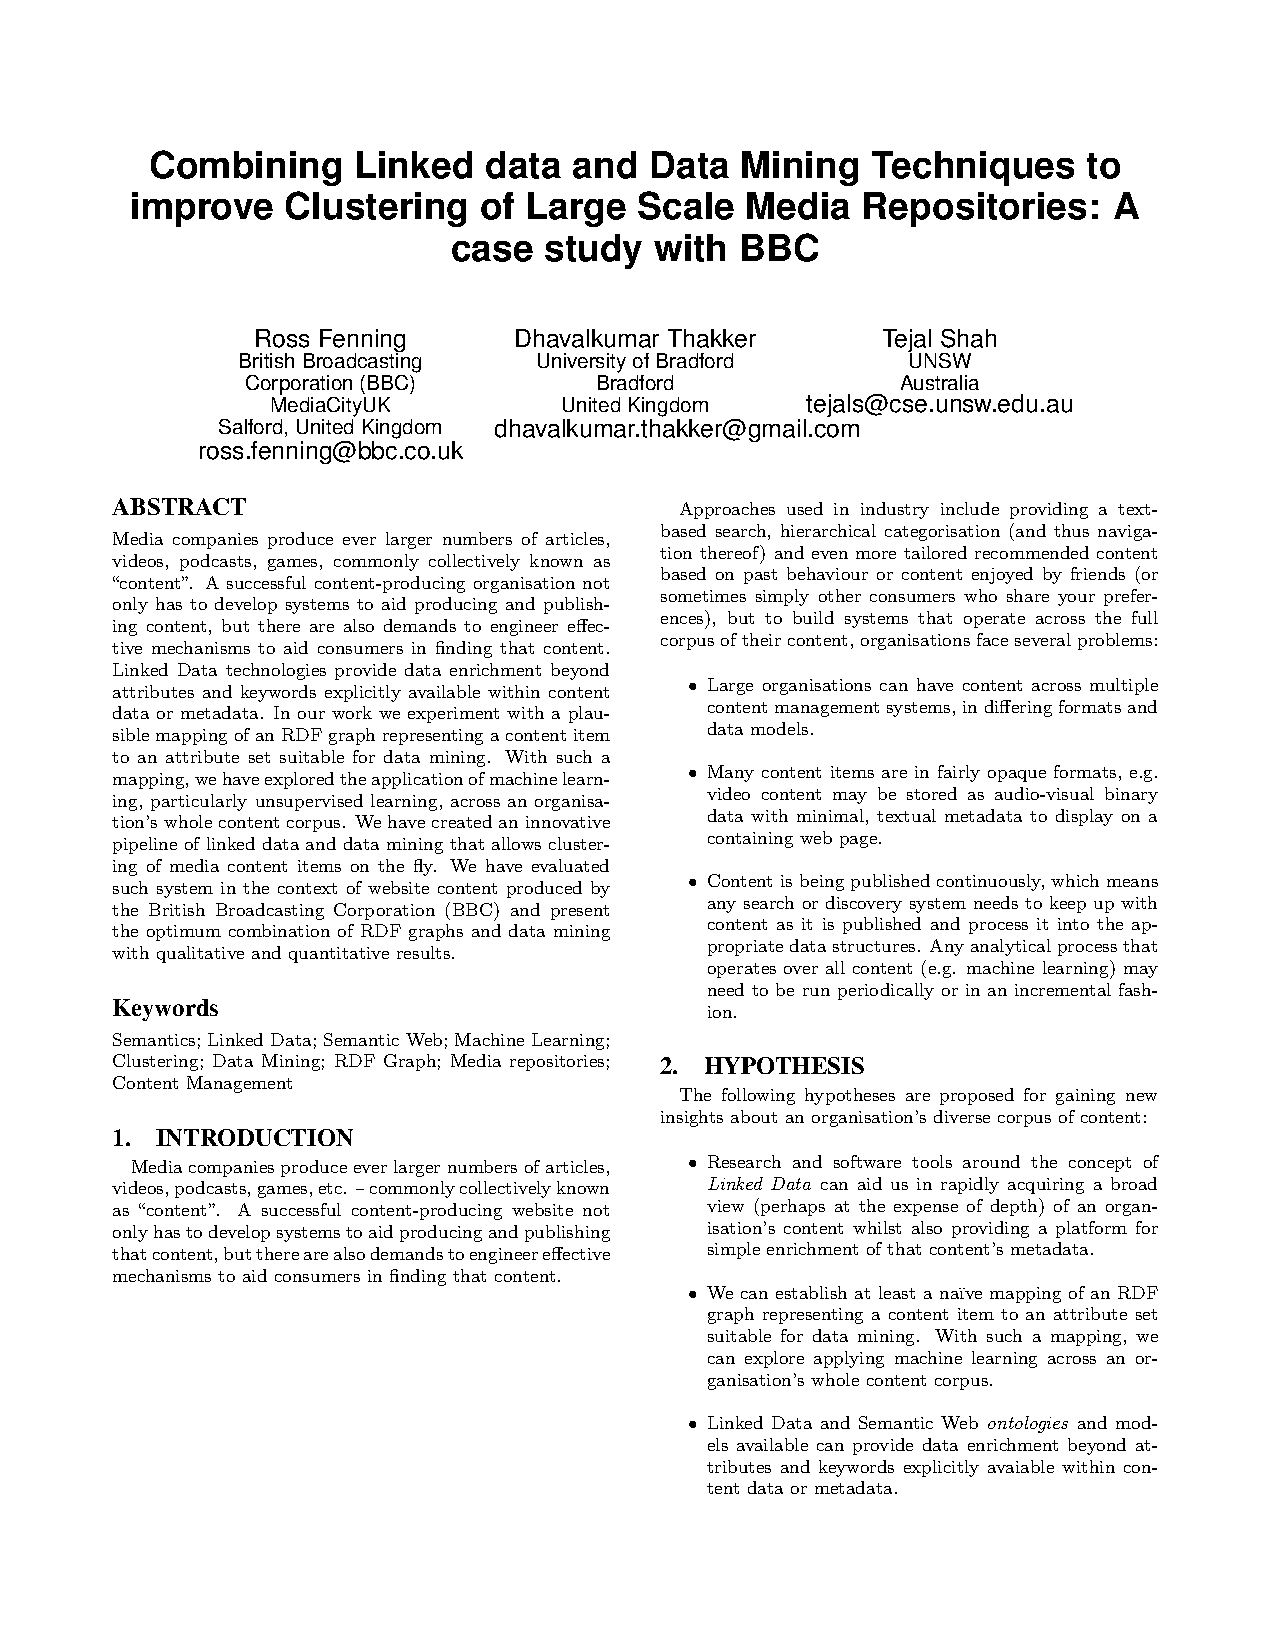
\includepdf{../paper/paper.pdf}

\end{document}
